% v1.04 - May 2023

\documentclass[]{interact}

\usepackage{epstopdf}% To incorporate .eps illustrations using PDFLaTeX, etc.
\usepackage{color} % doh

\usepackage{subfigure}% Support for small, `sub' figures and tables
%\usepackage[nolists,tablesfirst]{endfloat}% To `separate' figures and tables from text if required
\usepackage{longtable}
\usepackage{tabularx}
\usepackage{ltablex}  % This combines longtable and tabularx
\usepackage{colortbl}

\usepackage{gensymb}
\usepackage{multirow}

\usepackage{xcolor}

\usepackage{longtable}
\usepackage{tabularx}
\usepackage{booktabs}

\usepackage[hyphens]{url} % to break urls in bibliography
\usepackage[breaklinks=true]{hyperref} % LaTeX cross references become hyperlinks in pdf output


\usepackage{tikz} % Useful for drawing images, used for creating the frontpage
\usetikzlibrary{positioning} % Additional library for relative positioning 
\usetikzlibrary{calc} % Additional library for calculating within tikz

% Defines a command used by tikz to calculate some coordinates for the front-page
\makeatletter
\newcommand{\gettikzxy}[3]{%
  \tikz@scan@one@point\pgfutil@firstofone#1\relax
  \edef#2{\the\pgf@x}%
  \edef#3{\the\pgf@y}%
}
\makeatother

\usepackage{pdflscape}

\usepackage[square,sort&compress]{natbib}% Citation support using natbib.sty
\bibliographystyle{tfcad.bst} % Use the style of your choice   

\hypersetup{colorlinks=true,linkcolor=blue,urlcolor=blue}
\usepackage{soul}


\usepackage{longtable}
\usepackage{caption}
% what they recommend
\usepackage{array}
\usepackage{enumitem}
\usepackage{amssymb}
\usepackage[demo]{graphicx}
%\widowpenalty10000
%\clubpenalty10000 % to avoid sinle lines at the beginning or bottom of pages

\begin{document}

\articletype{Research Article}

\title{A Data-Driven Approach to Structural Vulnerability Assessment and Intervention Planning for Adobe Structures: A Case Study of Fort Union National Monument}

\author{
\name{Mina Savoroliya \textsuperscript{a}, Evan OJ \textsuperscript{b}, Frank Matero \textsuperscript{c}, Thomas Boothby \textsuperscript{a}, Rebecca Napolitano \textsuperscript{a}, \thanks{CONTACT Rebecca Napolitano. Email: nap@psu.edu}}
\affil{\textsuperscript{a}The Pennsylvania State University, Architectural Engineering Department, PA, USA}
\affil{\textsuperscript{b}NPS}
\affil{\textsuperscript{c}UPenn}
}

\maketitle

\begin{abstract}
This study presents a data-driven approach to assess structural vulnerability and develop intervention strategies for adobe structures, using Fort Union National Monument (FOUN) as a case study. The research integrates multiple analytical methods, including correlation analysis, Principal Component Analysis (PCA), and Random Forest machine learning, to identify and prioritize NSCs affecting adobe structure behavior. The study analyzed various degradation mechanisms, including adobe wall deterioration, foundation issues, shelter coat damage, and bracing problems. 
Data collection involved on-site surveys, archival research, LiDAR scanning. The analysis revealed key NSCs for each degradation category, such as cracking at wall junctions, foundation stone deterioration, and bracing angle issues. Based on these findings, intervention matrices were developed, incorporating preservation standards and durability estimates. 
The results demonstrate the effectiveness of this data-driven methodology in identifying vulnerabilities and guiding preservation strategies. The study provides a structured approach to prioritizing interventions, balancing historical preservation needs with structural integrity concerns. This methodology offers a framework for the assessment and preservation of adobe structures, potentially applicable to other historical sites facing similar challenges.

\end{abstract}

\begin{keywords}
adobe structures; structural vulnerability assessment; data-driven analysis; intervention planning; structural health monitoring
\end{keywords}

\section{Introduction}

Adobe structures, emblematic of the American Southwest's cultural heritage, represent a unique intersection of history and engineering \cite[]{houben2004}. 
Their earthen composition ties them intrinsically to their landscapes, yet also renders them vulnerable to environmental challenges \cite[]{richards2019, reyes2019, fuentes2019}.
The study of earth-based construction materials has seen significant advancements over the past two decades. 
Early research laid the groundwork for understanding these materials' structural properties. 
\cite[]{J2001} examined the reinforcement behavior of steel bars in cement-stabilized rammed earth, providing insights into reinforcement techniques. 
Building on this, \cite[]{Vasilios2008} investigated the compressive behavior of rammed earth structural elements, offering insights into load eccentricity and slenderness effects.
As the field progressed, durability became a key focus. 
\cite[]{Bui2009} investigated the durability of rammed earth walls, particularly when reinforced with natural hydraulic lime, demonstrating the material's ability to withstand natural weathering. 
This research was complemented by \cite[]{Fratini2011}, who characterized earth-based construction materials in historical structures, identifying optimal clay content for best mechanical performance.

The early 2010s saw a shift towards more sophisticated analysis methods. 
\cite[]{Ciancio2013} proposed a new method for analyzing the structural capacity of unreinforced rammed earth walls under lateral wind forces; \cite[]{Bui2014} focused on failure mechanisms of rammed earth walls, identifying stress concentrations at loaded zones as important considerations; \cite[]{Illampas2014} integrated laboratory testing with finite element simulations for more accurate structural evaluations under horizontal loading conditions, highlighting the influence of weak bonding between masonry units and mortar joints on seismic performance.
Long-term behavior and advanced modeling techniques became prominent in subsequent years. \cite[]{Bui2015} explored the aging and creep behavior of rammed earth, contributing to our knowledge of its long-term structural integrity. 
\cite[]{Bui2016} further advanced numerical analysis techniques by utilizing the discrete element method to simulate rammed earth behavior under various loading conditions.

Recent studies have investigated more specific aspects of earth-based materials. 
\cite[]{Characterization-mechanical} offered an overview of unstabilized rammed earth, examining aspects like compressive strength and thermal performance; \cite[]{non-industrial} examined the compression behavior of rammed earth, establishing a basis for understanding its mechanical response under varying loading conditions.
Environmental factors have also been a recent focus. \cite[]{Effectofmoisture} found that slight increases in moisture content did not significantly affect wall strength, while \cite[]{Impactofrelative} explored the effects of relative humidity changes on compacted earth's mechanical properties. 
Lastly, \cite[]{Ioannou} provided a stress-strain equation for adobe bricks, essential for structural design, further refining our understanding of these materials.

Seismic behavior has been a focus for several researchers. 
\cite[]{Varum2015} conducted in-depth studies on the mechanical properties of adobe units and mortars, performing strength and joint shear tests. 
\cite[]{Sathiparan2018} examined the importance of roof and diaphragm connectivity in seismic performance, revealing the benefits of PP-band retrofitting. \cite[]{Xekalakis2023} demonstrated how wooden ring beams significantly contribute to seismic resilience in adobe structures. 
\cite[]{Rafi2022} proposed a seismic strengthening scheme using steel wire mesh and cement-sand mortar, validated through shaking table tests.
\cite[]{hart2023} experimentally subjected extant adobe block construction walls to a local 100-year return interval rainfall intensity, highlighting the importance of data-driven modeling in targeting preservation methods effectively.

Data-driven approaches, particularly Principal Component Analysis (PCA) and correlation analysis, have gained prominence in structural health monitoring, offering new avenues for preservation and risk mitigation in historic adobe structures. 
The evolution of these techniques has significantly enhanced our ability to detect and analyze structural changes while accounting for environmental factors.
Early research in this field focused on developing methods to differentiate between environmental effects and actual structural damage. 
\cite[]{Yan2005} introduced a PCA-based method for detecting structural damage that integrated environmental factors without direct measurement. 
They further refined this concept in a subsequent study \cite[]{Yan2005b}, applying local PCA in a clustered data environment to address non-linear complexities. 
This work laid the foundation for more sophisticated analysis techniques in structural health monitoring.
Building on these advancements, \cite[]{Bellino2010} demonstrated PCA's effectiveness in both Linear Time-Invariant and Linear Time-Varying systems. 
Through experiments on a clamped-free beam and numerical simulations of a train crossing a railway bridge, their work showcased PCA's ability to discern damage from environmental influences, further validating its utility in structural health monitoring.

The application of these techniques to real-world structures was exemplified by \cite[]{Magalhães}, who analyzed data from a concrete arch bridge in Porto. 
They employed static and dynamic regression models enhanced by PCA to establish relationships between natural frequencies and influencing factors, demonstrating the practical application of these methods in complex, real-world environments.
In the realm of vibration-based structural health monitoring, \cite[]{Ubertini2013} implemented a system for the San Pietro belltower in Perugia. 
Using ambient vibration tests and machine learning methods including PCA, they were able to identify post-earthquake anomalies in structural behavior. Their approach, which employed novelty analysis for damage detection, showcased the potential of these techniques in preserving historic structures.

More recently, \cite[]{Zucconi2017} expanded the application of PCA to large-scale scenario analysis. 
They developed a model to predict the habitability of unreinforced masonry buildings post-earthquake, utilizing PCA to analyze over 60,000 buildings and identify seven parameters impacting usability. 
This study demonstrated the potential of machine learning techniques for scenario analysis and planning in regions with similar building characteristics, highlighting the scalability of these methods.

As technology continues to advance, these methods are likely to play an increasingly important role in safeguarding not only civil infrastructure but also our architectural heritage.
In the realm of preservation, \cite[]{Dehghan} used PCA to assess the effectiveness of historic buildings repurposed as boutique hotels. 
Their study distilled 24 indicators into three principal components, providing actionable insights for stakeholders in making user-centric improvements.
This study demonstrates the power of data-driven techniques in enhancing our understanding and management of historic structures, offering new tools for preservation and risk mitigation.

\section{Research aim}

This study aimed to develop and validate a data-driven approach for assessing structural vulnerability and creating effective intervention plans for adobe structures, using FOUN as a case study. 
Specifically, we addressed the following research questions:
(1) How can data-driven analysis techniques, including correlation analysis, PCA, and Random Forest machine learning, be effectively applied to identify and prioritize %TEB. 
 This is the first time this term comes up.  It would be a good time to explain exactly what you mean. '??The objective of this investigation is to find the necessary and sufficient conditions (Harris) associated with the observed damage, e.g. water ingress is an NSC for adobe erosion or settlement is an NSC for wall leaningNSCs affecting adobe structure behavior? 
(2) To what extent can these data-driven methods enhance our understanding of the complex interrelationships between various degradation mechanisms in adobe structures?
(3) How can the insights gained from data-driven analysis be translated into practical, prioritized intervention strategies that balance historical preservation needs with structural integrity concerns?
By addressing these questions, this study sought to bridge the gap between traditional preservation methods and modern data analysis techniques, offering a new framework for the assessment and preservation of adobe structures. 
The results demonstrate how data-driven approaches can lead to more informed, efficient, and effective preservation strategies.

\section{Case study}

\begin{figure}[h]
    \centering
\includegraphics[width=1\textwidth]{Images/FOUN.png}
    \caption{Fort Union National Monument \cite[]{map}}
    \label{fig:whole_site}
\end{figure}

FOUN is a historically significant site adjacent to the historic Santa Fe Trail. It was established in 1851, shortly after New Mexico became a U.S. territory. Over its history, three distinct structures were built in proximity, each serving a different strategic purpose. This study focuses on the hospital building located at the southeast end of the site, which is part of the third instance of Fort Union (Figure~\ref{fig:whole_site}). 

\begin{figure}[h]
    \centering
\includegraphics[width=0.8\textwidth]{Images/land.png}
    \caption{FOUN site plan \cite[]{map}}
    \label{fig:whole_site}
\end{figure}

The Third Fort hospital at FOUN was constructed between late 1863 and early 1864 and remained in use until 1891 when the last soldiers left for Fort Wingate and while Fort Union was vacated. 
Since its abandonment in 1891, the hospital complex (Figure~\ref{fig:fort_union_hospital_plan}), along with the rest of the fort, has been subject to various environmental and human-induced challenges. 
These include exposure to the elements, natural deterioration processes, and periods of limited maintenance before its designation as a National Monument. 
The site also experienced some salvage of materials prior to NPS management.

\begin{figure}[h!]
    \centering
    \includegraphics[width=0.8\textwidth]{Images/hospital.png}
    \caption{The plan of hospital at FOUN}
    \label{fig:fort_union_hospital_plan}
\end{figure}

Since the 1950s the National Park Service (NPS) has made continual efforts to stabilize the remnant walls, including an array of wall bracings and other supports, but certain problems with the walls require unusual efforts to maintain them in place and preserve the remaining original fabric. The hospital complex includes the hospital itself, the inner courtyard, and areas enclosed by the surrounding compound wall foundations and exterior to the hospital and inner courtyard. 

\section{Materials and methods}
\subsection{Data collection}
\subsubsection{For adobe walls}
The dataset documents adobe structural damage at FOUN. Each entry represents a wall section identified by a unique ID and includes features and scores reflecting the condition of the adobe structures. 
Data sources include photographic documentation, Lidar scans, architectural plans provided by the National Park Service, and archival research identifying past treatment efforts. 
Data was collected using a rapid assessment survey (RAS), complemented by an illustrated glossary.
Figure~\ref{fig:RASsample} shows a sample of this illustrated glossary, and additional information can be found in Section \ref{sec:ras}.

\begin{figure}[h!]
    \centering
    \includegraphics[width=1\textwidth]{Images/RASsample.png}
    \caption{Example pages from the illustrated glossary that accompanied the RAS}
    \label{fig:RASsample}
\end{figure}

The dataset includes the following features, each with an associated scoring system to quantify the level of damage or presence of specific attributes. 
Definitions about orientation can be found in Section \ref{sec:orient}. 
\begin{itemize}
    \item \textbf{Coat Cracking (Orientations 1 \& 2):}  Represents the level of cracking in the shelter coat.
        \begin{itemize}
            \item 0: No Damage
            \item 1-5: Damage Level (increasing severity)
        \end{itemize}
    \item \textbf{Coat Loss (Orientations 1 \& 2):} Represents the level of loss in the shelter coat.
        \begin{itemize}
            \item 0: No Damage
            \item 1-5: Damage Level (increasing severity)
        \end{itemize}
    \item \textbf{Structural Cracking:} Represents the presence and severity of structural cracks.
        \begin{itemize}
            \item 0: No Damage
            \item 1-5: Damage Level (increasing severity)
            \item 6: Wall Destroyed
        \end{itemize}
    \item \textbf{Cracking at Wall Junction:} Represents the presence and severity of cracks at wall junctions.
        \begin{itemize}
            \item 0: No Damage
            \item 1-5: Damage Level (increasing severity)
            \item 6: No Wall Junction
        \end{itemize}
    \item \textbf{Lintel Deterioration:} Represents the condition of the lintel (if present).
        \begin{itemize}
            \item 0: No Damage
            \item 1-5: Damage Level (increasing severity)
            \item 6: No Lintel
        \end{itemize}
    \item \textbf{Foundation Displacement (Elevations 1 \& 2):} Represents the displacement of the foundation.
        \begin{itemize}
            \item 0: No Damage
            \item 1-5: Damage Level (increasing severity)
            \item -1: Missing Data
        \end{itemize}
    \item \textbf{Foundation Mortar Condition (Elevations 1 \& 2):} Represents the condition of the mortar in the foundation.
        \begin{itemize}
            \item 0: No Damage
            \item 1-5: Damage Level (increasing severity)
            \item -1: Missing Data
        \end{itemize}
    \item \textbf{Sill (Orientations 1 \& 2):} Represents the condition of the sill (if present).
        \begin{itemize}
            \item 0: No Sill
            \item 1-5: Damage Level (increasing severity)
            \item 6: Sill Destroyed
        \end{itemize}
    \item \textbf{Cap Deterioration:} Represents the condition of the wall cap (if present).
        \begin{itemize}
            \item 0: No Cap
            \item 1-5: Damage Level (increasing severity)
            \item 6: Wall Destroyed
        \end{itemize}
    \item \textbf{Surface Loss at Top, Mid, and Low Level:} Represents the level of surface erosion at different wall levels.
        \begin{itemize}
            \item 0: No Damage
            \item 1-5: Damage Level (increasing severity)
        \end{itemize}
    \item \textbf{Out of Plane:} Represents the degree to which the wall is leaning or racked.
        \begin{itemize}
            \item 0: No Damage
            \item 1-5: Damage Level (increasing severity)
        \end{itemize}
    \item \textbf{Height:} Represents the remaining height of the wall.
        \begin{itemize}
            \item 1: No Damage (Full Height)
            \item 2-5: Damage Level (decreasing height)
        \end{itemize}
    \item \textbf{Foundation Height:}  Represents the exposed height of the foundation in inches. A blank cell indicates the foundation is not exposed.
    \item \textbf{Animal Activity:} Represents the level of animal activity.
        \begin{itemize}
            \item 0: No Damage
            \item 1-5: Damage Level (increasing severity)
        \end{itemize}
    \item \textbf{Foundation Stone Deterioration:} Represents the condition of the foundation stones.
        \begin{itemize}
            \item 0: No Damage
            \item 1-5: Damage Level (increasing severity)
            \item -1: Missing Data
        \end{itemize}
    \item \textbf{Bracing Score:} Represents the condition of any bracing present.  Calculated based on observed damage to the bracing.
        \begin{itemize}
            \item 0: No Bracing
            \item 1-5: Damage Level (decreasing condition)
        \end{itemize}
    \item \textbf{Fireplace:} Indicates the presence and proximity of a fireplace.
        \begin{itemize}
            \item 0: No Fireplace
            \item 1: Has Fireplace
            \item 2: Adjacent Fireplace
        \end{itemize}
    \item \textbf{Treatment:} Indicates whether the section has undergone treatment.
        \begin{itemize}
            \item 0: Not Treated
            \item 1: Treated
        \end{itemize}
    \item \textbf{Bracing:} Indicates the presence of bracing.
        \begin{itemize}
            \item 0: No Bracing
            \item 1: Has Bracing
        \end{itemize}
    \item \textbf{Point Cloud Deviation:} Standard deviation of the foundation's surface points relative to a reference plane. A smaller standard deviation suggests uniform, consistent behavior in foundation blocks' alignment with the reference plane. A larger standard deviation indicates more variability in alignment differences.
    \item \textbf{Point Cloud Mean:} Average vertical position of the foundation's surface relative to a reference plane. A smaller mean deviation means the foundation block closely matches the reference plane, suggesting a flat ground surface. A larger mean deviation indicates more unevenness or irregularities beneath the block.
\end{itemize}

\subsubsection{For bracing}

Data collection for bracing elements involved on-site assessments and examining engineering documentation (Section \ref{sec:bracing}).
The following features were recorded for each bracing element:

\begin{itemize}
    \item \textbf{Angle from Horizontal:} Whether the bracing angle was greater than 60 degrees from the horizontal.
    \item \textbf{Slack Braces:} Presence of slack or looseness in the bracing element.
    \item \textbf{Wood Deterioration in Anchor:} Presence and extent of wood deterioration in the bracing anchor.
    \item \textbf{Lack of Effective Fasteners in Anchor:} Assessment of the adequacy and condition of fasteners used in the bracing anchor.
    \item \textbf{Single or No Contact Point in Pad:} Whether the bearing pad had only a single contact point or no contact with the wall.
    \item \textbf{Wood Deterioration in Brace:} Presence and extent of wood deterioration in the bracing element itself.
    \item \textbf{Bearing Pad Evidently Pushed Through:} Evidence of the bearing pad having pushed through the wall material.
\end{itemize}

These individual observations were then synthesized into quantitative metrics to facilitate statistical analysis. 
A ‘bracing score’ was calculated for each bracing element. 
Each bracing began with a base score of 5, from which points were deducted based on the presence and type of observed damage. 
Each damage type was assigned a value of 1, simplifying the scoring process by treating each damage occurrence equally. 
The ‘bracing score’ thus reflected the overall condition of the bracing element. 
For walls with multiple bracings, an ‘average bracing score’ was calculated to assess the overall condition of bracing elements for each wall section, accounting for variations in the number of bracings present.

\subsection{Analysis methods}
The Pearson Correlation was initially employed to explore the linear interrelationships among the various parameters influencing adobe structure behavior. 
By calculating Pearson correlation coefficients for each pair of parameters, we quantified the strength and direction of linear relationships. 
Coefficients approaching +1 or -1 indicated strong positive or negative linear associations, respectively, while values near 0 suggested a negligible linear relationship. 
This process yielded a correlation matrix, providing a comprehensive overview of the linear interdependencies between all parameter pairs. To ensure the robustness of our findings, we also calculated p-values for each correlation coefficient. 
A small p-value (e.g., p < 0.05) indicated strong evidence against the null hypothesis (no correlation), suggesting that the observed correlation was statistically significant and unlikely due to random chance. 
We then focused on interpreting the statistically significant correlations, moving beyond simply identifying the 'what' to understanding the 'why' behind these relationships. 
This involved analyzing the context of each correlation to discern the underlying theoretical or practical reasons driving the observed association, thereby translating statistical findings into actionable insights for decision-making.

PCA is a dimensionality reduction technique that transforms a dataset with potentially correlated variables into a new set of uncorrelated variables called principal components. 
These components are ordered by the amount of variance they explain in the original data. 
The first principal component captures the most variance, the second captures the second most, and so on. 
By focusing on the first few principal components, which explain the majority of the variance, we can reduce the complexity of the dataset while retaining the most important information. 
While Pearson correlation identifies linear relationships between pairs of variables, PCA takes a more holistic approach. 
Correlation assesses the association between two variables at a time, whereas PCA considers all variables simultaneously to identify underlying patterns and reduce the dimensionality of the data. 
In essence, correlation looks at individual links, while PCA looks at the overall structure of the network of relationships. 
PCA serves as a complement to correlation analysis for several reasons. First, PCA can reveal underlying structures and relationships that might be obscured by the pairwise nature of correlation analysis. 
Second, PCA can handle multicollinearity (high correlation between multiple variables), which can complicate the interpretation of correlation coefficients. 
By reducing the dimensionality of the data, PCA simplifies the analysis and allows us to focus on the most influential factors driving adobe structure behavior. 
Finally, PCA can help identify latent variables (principal components) that represent combinations of original variables, providing a more comprehensive understanding of the complex interactions affecting adobe degradation. 
For example, a principal component might represent a combination of moisture content, temperature fluctuations, and shelter coat condition, providing a single measure of overall environmental stress.

Building upon the insights gained from both correlation analysis and PCA, we further refined our understanding by employing Random Forest. 
While PCA effectively reduced the dimensionality of the data and identified key underlying factors, it primarily focuses on explaining variance and does not directly predict specific outcomes or classify structures based on their vulnerability. 
Random Forest, in contrast, is a supervised learning algorithm capable of modeling complex, non-linear relationships between predictor variables and a target variable (e.g., the degree of adobe wall deterioration, the presence of foundation cracking, or the severity of shelter coat damage). 
This predictive capability allowed us to not only identify the most important factors contributing to degradation but also to estimate the likelihood of specific degradation outcomes under different conditions. 
Random Forest offers several advantages in this context. 
First, it is robust to multicollinearity, a common issue in environmental and material science data, which can be further mitigated by the prior application of PCA. 
Second, it can handle both continuous and categorical predictor variables. 
Third, it provides measures of variable importance, allowing us to rank the factors most influential in predicting degradation. 
Finally, Random Forest is relatively resistant to overfitting, making it suitable for complex datasets with a moderate number of observations. 

\subsection{Data synthesis methods}
Intervention matrices graphically represent the logic of intervention decisions, reminding stakeholders to consider multiple perspectives and options\cite[]{harris2001building}. The tool avoids formulaic responses to commonly encountered deterioration mechanisms by facilitating a structured evaluation of the various options, weighing their advantages and disadvantages, and considering cost, risk, efficacy, and potential outcomes. It also illustrates the complexity of decision-making in these contexts \cite[]{harris2001building}. In these matrices, the horizontal axis represents the NSC, while the vertical axis represents various intervention approaches, such as repointing mortar joints, installing a new shelter coat, improving drainage around the foundation, or adding structural bracing. The cells within the matrix represent a qualitative assessment of the effectiveness, cost, and potential risks associated with each intervention approach for a given NSC. For example, a cell might indicate that repointing mortar joints is highly effective for addressing cracking at wall junctions but has a moderate cost and a low risk of negatively impacting the historical fabric.
The initial step in developing an intervention matrix involves determining the NSCs.
This process uses the outputs of ranked Pearson correlations, PCA, and Random Forest to identify which features show the strongest associations with others.  

\section{Results and discussion}

\subsection{Understanding damages to adobe walls}
%TEB. I would simply remove the heatmap figures and boil 5.1.1 down to a tabular summary of the correlations with p<0.5.  The figures are long, hard to read and distract from the later results

\subsubsection{Correlation Analysis for Damage to Adobe Walls}
Creating a heatmap derived from the calculated correlation coefficients was our primary method in the visualization for this analysis. It employs varying color intensities to depict the strength of the correlations, offering an immediate, intuitive grasp of how each parameter relates to the others.  Figure~\ref{figure:correlation-matrix-heatmap} displays the complete heatmap. For greater clarity, the heatmap has been divided into three sections, as depicted in Figures ~\ref{figure:heatmap1} to~\ref{figure:heatmap3}. 
%%%
\begin{figure}[h]
    \centering
    \includegraphics[width=1\textwidth]{Images/heatmap5.png}
    \caption{Correlation matrix heatmap}
    \label{figure:correlation-matrix-heatmap}
\end{figure}
%%%
\clearpage

\begin{landscape}
 %%%
\begin{figure}[h!t]
    \centering
    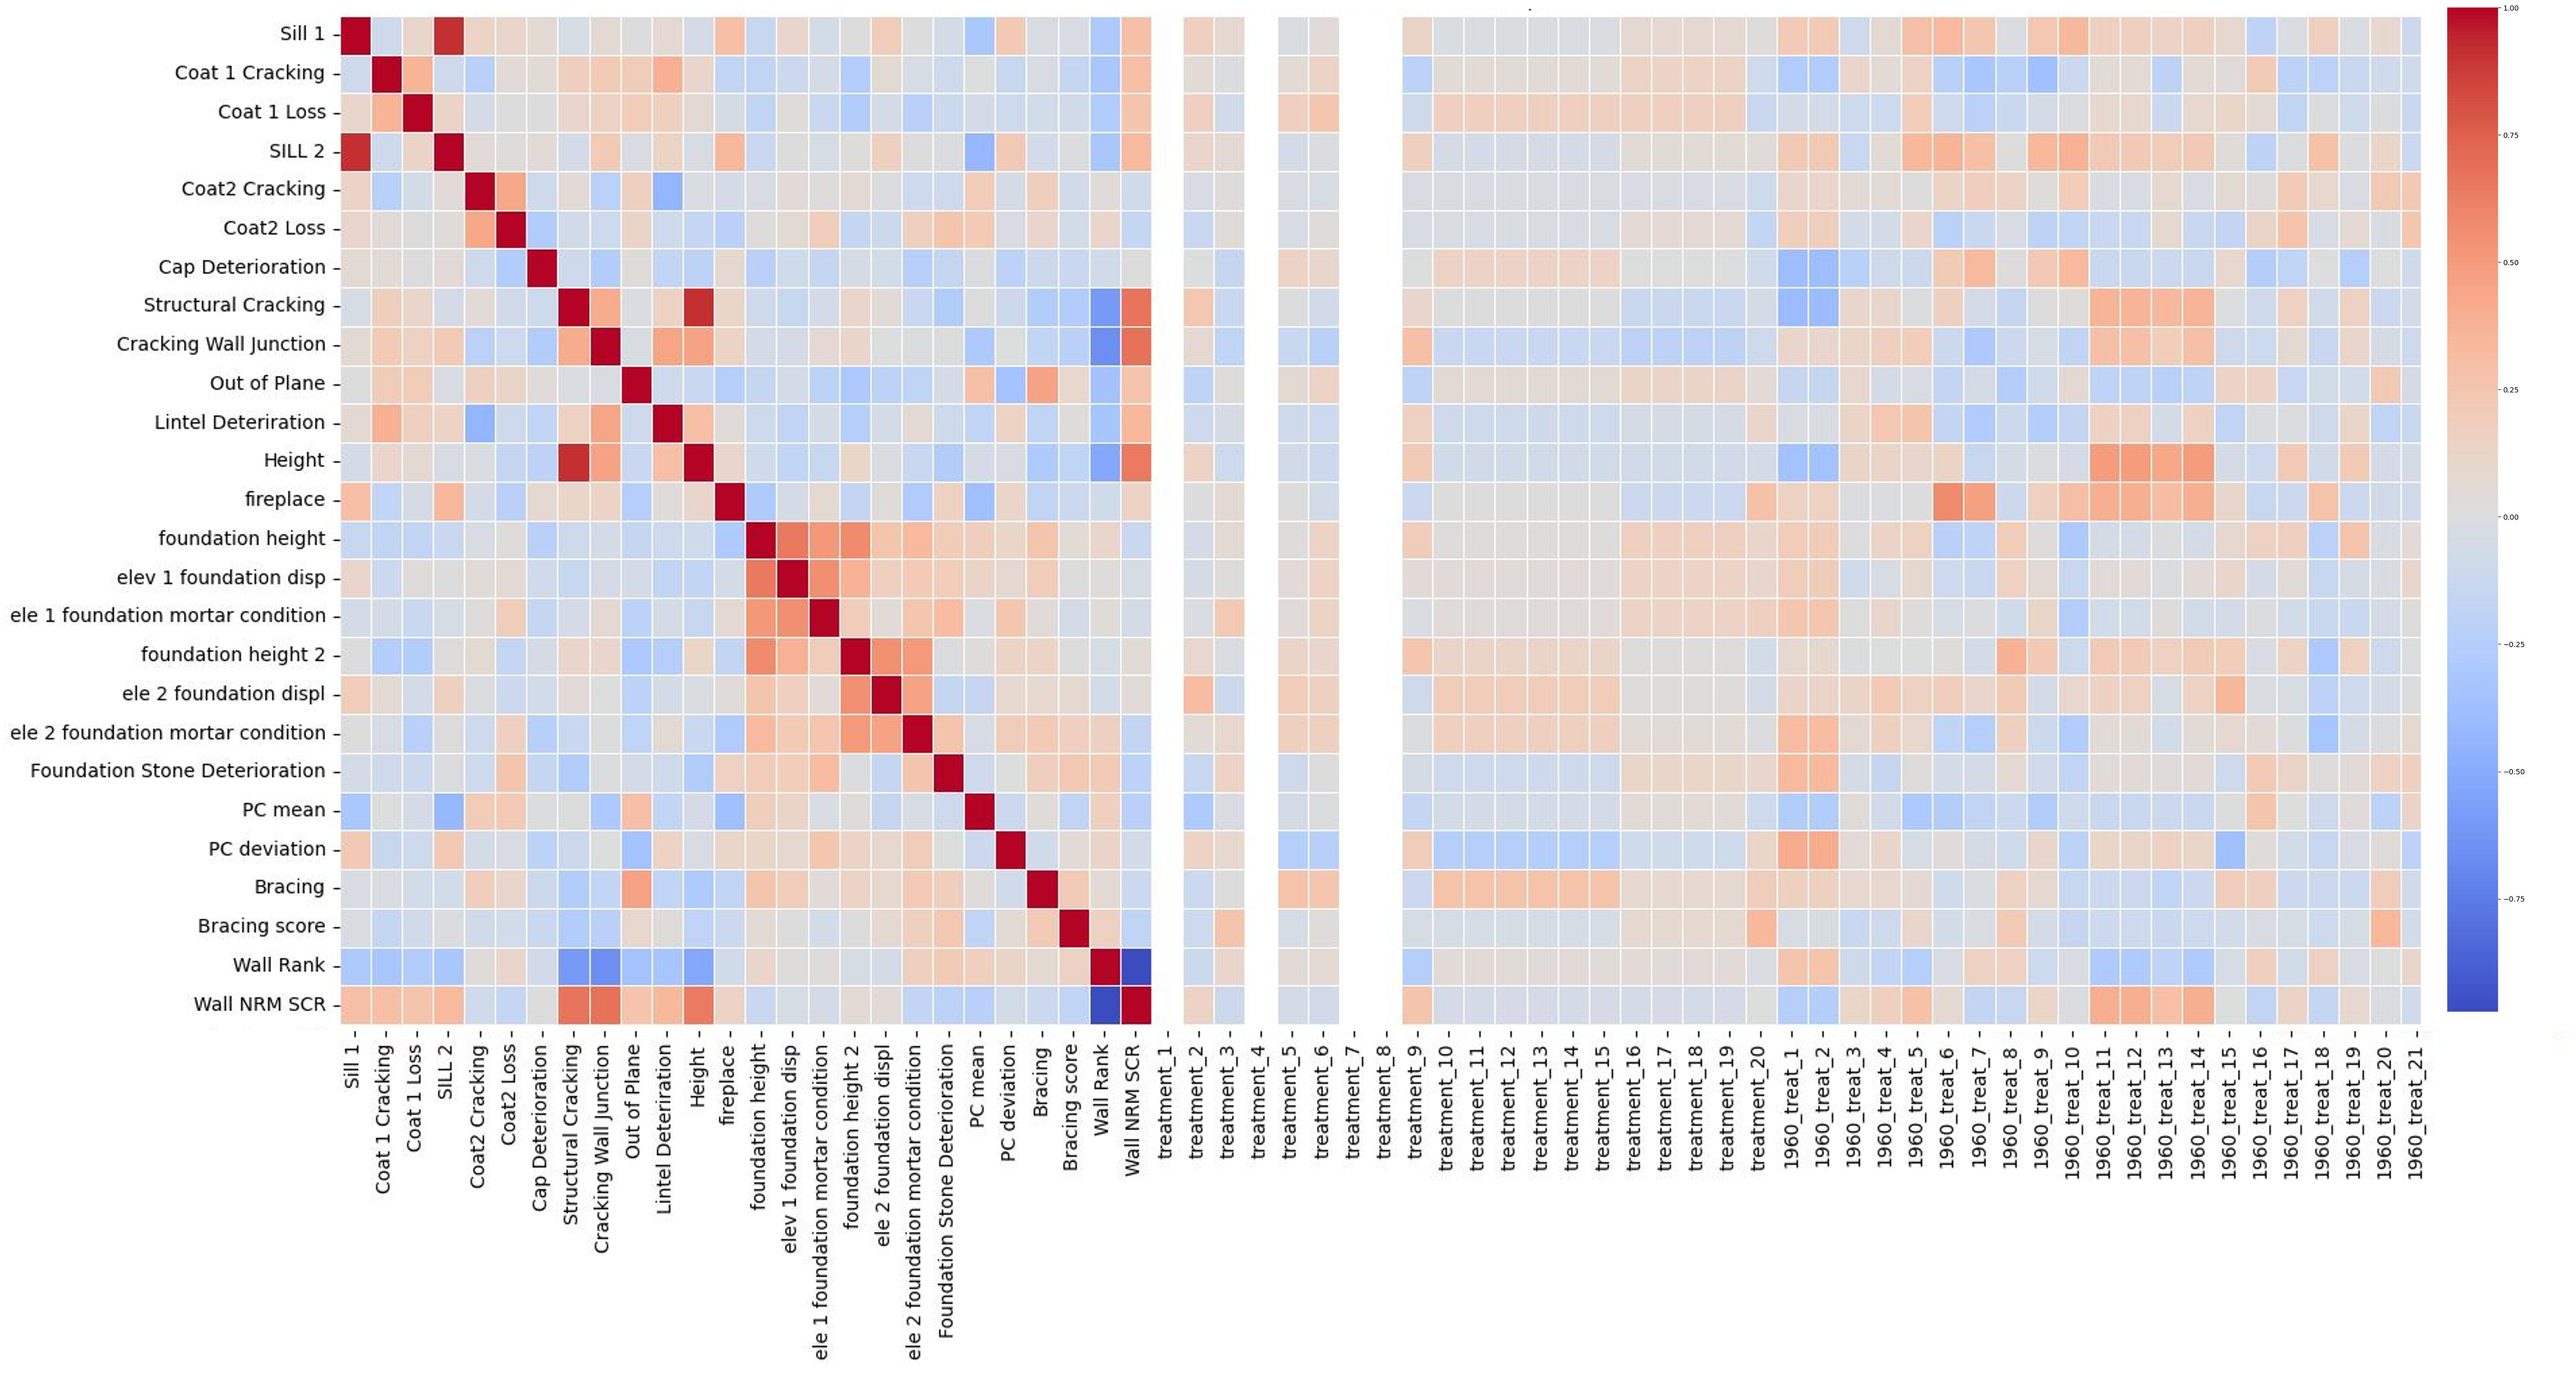
\includegraphics[scale=.7]{Images/heat1.png}
    \caption{Correlation matrix heatmap part 1}
    \label{figure:heatmap1}
\end{figure}
%%%   
\end{landscape}

\begin{landscape}
 %%%
\begin{figure}[h!t]
    \centering
    \includegraphics[scale=.7]{Images/heatmap2.png}
    \caption{Correlation matrix heatmap part 2}
    \label{figure:heatmap2}
\end{figure}
%%%   
\end{landscape}

\begin{landscape}
 %%%
\begin{figure}[h!t]
    \centering
    \includegraphics[scale=.7]{Images/heatmap4.png}
    \caption{Correlation matrix heatmap part 3}
    \label{figure:heatmap3}
\end{figure}
%%%   
\end{landscape}


Using the correlation analysis and its heatmap representation, we concentrated on identifying strong correlations that could have a significant impact. When calculating correlations, we also calculated p-values for each correlation coefficient.
This statistical significance threshold ensured that the relationships we considered were statistically strong and less likely to result from random chance.
The next phase was to investigate the interpretation of the correlations, understanding not just the 'what' but the 'why' behind these relationships. 
This stage was pivotal in translating statistical findings into meaningful insights that could guide our decision-making and model development processes.
We approached this by analyzing the context of each correlation; this involved understanding the theoretical or practical reasons.

For example, we observed significant correlations between conditions affecting foundation degradation, giving us insights into the impact of environmental conditions on structural integrity. 
The foundation exposed height showed positive correlations with foundation mortar condition in both elevations (correlation of 0.329 with p-value 0.00647 for Elevation 2, and 0.508 with p-value 1.13E-05 for Elevation 1). 
Additionally, foundation stone deterioration correlated with coat loss in Orientation 2 (correlation of 0.258 with p-value 0.0343). 
These correlations suggest that exposure to weather leads to more deterioration, with the link between foundation stone deterioration and coat loss attributed to weathering effects.

Another example of a correlation was between 'lintel deterioration' and treatment. There is a negative correlation (correlation of -0.252 with p-value 0.0393) between 'lintel deterioration' and 'rebuilt or missing foundations.' FOUN hospital has 69 sections among these, 45 sections have lintels, with nearly half (22) receiving treatment; 36\% of the treated sections are destroyed, compared to 61\% of the untreated ones, suggesting better performance of lintels in sections without the treatment.

Conversely, 'add vertical support' correlated positively with 'lintel deterioration' (correlation of 0.242 with p-value 0.0480), exacerbating the issue. 
All six lintels in the seven sections with added supports are destroyed, indicating a potential adverse effect of vertical supports on lintel integrity. 
This is contrasted by 17 other destroyed lintels in sections without such supports, further emphasizing the negative impact of added supports.

Another correlation we examined was between 'sill deterioration' and 'rebuilt missing foundation'. 
Sill deterioration in both orientations showed positive correlations with rebuilt missing foundation (Sill 1: correlation of 0.241 with p-value 0.0485; Sill 2: correlation of 0.342 with p-value 0.00450). 
Among 69 analyzed sections, 37 have a sill, with 20 undergoing treatment and showing signs of deterioration — this represents 54\% of the section with sill. In contrast, the 17 untreated sections with sills comprising 46\% also show deterioration. The treatment likely exacerbated the sill deterioration.

We also found a correlation between 'cracking at wall junction' with 'structural cracking' (correlation of 0.291 with p-value 0.0166). 
In 67\% of all sections (46 sections), a structural crack also exists when there is a crack at the wall junction. It may be that the same conditions create structural cracking and cracking at the wall junction.

The correlation values between 'out of plane' and both 'point cloud deviation' and 'point cloud mean' uncover significant patterns in structural behavior. 
A negative correlation between 'out of plane' and 'point cloud deviation' (correlation of -0.341 with p-value 0.0047) indicates that sections are more likely to move out of the plane when the foundation deformations are more uniform. 
Meanwhile, the positive correlation between 'out-of-plane' and 'point cloud mean' (correlation of 0.285 with p-value 0.0192) suggests that foundation displacement could play an important role in causing these shifts, with walls experiencing more significant displacement being more susceptible to moving out of the plane.

'Sill deterioration' is correlated with other conditions and treatments. The relationship between 'sill deterioration' and 'point cloud mean' reveals essential insights. 
A negative correlation (Sill 1: correlation of -0.307 with p-value 0.0112; Sill 2: correlation of -0.418 with p-value 0.0004) suggests that sill deterioration may be significantly influenced by foundation displacement, indicating that foundation shifts could exacerbate sills' deterioration.

In the subsequent sections, we investigated a series of correlations identified as significant within our analysis, but they were misleading. 
For instance, the correlation between 'structural cracking' and 'lintel deterioration' (correlation of -0.253 with p-value 0.03884) appeared unreasonable upon initial review. 
Five walls in the building are destroyed and hold a structural crack score of 0. 
It is possible that these walls had existing cracks contributing to the lintel destruction, thereby leading to a misleading correlation.
We also found correlations between 'fireplace' and 'sill' conditions, as well as various fireplace-related treatments and sill conditions. For example, 'fireplace' correlated with 'Sill 1' (correlation of 0.294 with p-value 0.01549) and 'Sill 2' (correlation of 0.341 with p-value 0.00464). 
While these correlations exist, the fireplace is remote from the sill, and there is unlikely to be a causal mechanism.
The relationship between 'lintel deterioration' and 'wall height' (correlation of -0.296 with p-value 0.0148) was also examined. 
Despite the negative correlation, the predominance of full-height walls and a lack of substantial evidence render this correlation insignificant.
Lastly, we investigated the correlation between 'height' and 'foundation stone deterioration' (correlation of 0.258 with p-value 0.0345). 
While there appears to be a connection between height and foundation stone deterioration, the fact that most walls (59 out of 69) have a uniform full height raises doubts about height's significance in assessing foundation condition. 
Since the foundation score mainly indicates stone deterioration, the idea that higher walls lead to more foundation problems seems less credible.


\subsubsection{PCA for adobe walls}

We calculated the cumulative explained variance to determine the optimal number of principal components required for our analysis. 
The cumulative explained variance is a measure that helps in understanding how much information (variance) is captured by the first few components. 
We identified a point of inflection that suggested eight principal components were sufficient to capture most of the variance in our data.

The PCA and heatmap interpretation provided an understanding of the dataset's structure, emphasizing different combinations and associations of variables across the components. This heatmap is shown in Figure \ref{fig:pca_heatmap} and Table \ref{tab:pca_summary} shows the summary of the PCA result. PCA was conducted for all variables, but the information displayed on the heatmap has been reduced to enhance visual clarity.

\begingroup
    \footnotesize
    \setlength\tabcolsep{4pt}
    \begin{longtable}{>{\raggedright\arraybackslash}p{2.5cm} p{11cm}}
        \caption{Summary of PCA findings after excluding wall rank.}
        \label{tab:pca_summary} \\  % Add caption here
        \toprule
        \textbf{Components} & \textbf{Constituents} \\
        \midrule
        \endfirsthead

        \multicolumn{2}{c}{\centering \tablename\ \thetable\ -- \textit{Continued from previous page}} \\  % Centering Here
        \toprule
        \textbf{Components} & \textbf{Constituents} \\
        \midrule
        \endhead

        \midrule
        \multicolumn{2}{r}{\textit{Continued on next page}} \\
        \endfoot

        \bottomrule
        \endlastfoot

        0 & Foundation Height 1, Foundation Height 2 \\
        \midrule
        1 & Foundation Height 1, Foundation Height 2 \\
        \midrule
        2 & Cracking at the Wall Junction, Structural Cracking, Lintel Deterioration, Height \\
        \midrule
        3 & Sill 1 and 2, Structural Cracking, Lintel Deterioration, Structural Cracking, Bracing Score, Foundation Mortar Condition in Elevation 2, Sill 1 \\
        \midrule
        4 & Lintel Deterioration, Structural Cracking, Bracing Score, Foundation Mortar Condition in Elevation 2, Sill 1 Deterioration \\
        \midrule
        5 & Cracking at Wall Junction, Foundation Mortar Condition 1, Lintel Deterioration, Foundation Displacement 2, Bracing Score, Height, Structural Cracking, Foundation Stone Deterioration \\
        \midrule
        6 & Foundation Mortar Condition in Elevations 1 and 2, Out of Plane, Cracking at Wall Junction, Structural Cracking, Cap Deterioration \\
        \midrule
        7 & Out of Plane, Cap Deterioration, Lintel Deterioration, Bracing Score \\
    \end{longtable}
\endgroup

\normalsize
\subsubsection{Random Forest for adobe walls}

While we were aware of the parameters used to calculate 'wall rank,' our objective was to identify if there were additional related parameters that could be considered for future iterations or inclusion in analyses of additional sites. The feature importance plot generated from this analysis, shown in Figure \ref{fig:random_forest}, represents feature significance. Random Forest analysis was conducted for all variables, but the information displayed on the Figure \ref{fig:random_forest}, has been reduced to enhance visual clarity.

\begin{figure}[h]
    \centering
    \includegraphics[width=0.95\textwidth]{Images/random_forest_plot.png}
    \caption{Random Forest analysis plot.}
    \label{fig:random_forest}
\end{figure}

The results showed that several variables not explicitly included in the calculation had a significant effect on wall rank. These variables include foundation stone deterioration, point cloud mean values, foundation mortar condition in elevation 1, point cloud deviation, foundation height in elevation 2, sill condition in orientation 1, and foundation displacement in elevation 1, listed in order of their impact. The results from the Random Forest analysis confirm our PCA findings, confirming that certain features are more critical in explaining the variations in 'wall rank.'



\subsection{Understanding damages to bracing}
%TEB similar comment here.  The heatmap itself doesn't show very much
\subsubsection{Correlation Analysis for Damage to bracing}
Additional analysis was employed to explore the relationships between various parameters that influence the behavior of bracings in adobe structures. This involved processing data on specific types of damage and characteristics of bracing observed at FOUN Hospital including ‘angle greater than 60° from horizontal’, ‘slack braces,’ ‘wood deterioration in anchor,’ ‘lack of effective fasteners in anchor,’ ‘single or no contact point in pad,’ ‘wood deterioration in brace,’ ‘bearing pad evidently pushed through.’ 
Pearson correlation analysis was conducted on bracing data to explore the linear relationships between the damages. The outcome was a heatmap shown in Figure~\ref{fig:Bheat}, generated to visually display these relationships, providing a view of the correlation among the parameters. 

\begin{figure}[h!]
    \centering
    \includegraphics[width=0.8\textwidth]{Images/bracingheatmap.png}
    \caption{Correlation matrix heatmap for bracing analysis }
    \label{fig:Bheat}
\end{figure}

Notably, a correlation exists between the presence of wood bracing and wall rank (correlation value: 0.2056), indicating increased wall damage in sections where wood bracing is present. 
Additionally, the condition of the bearing pad being evidently pushed through (correlation value: 0.3251), along with wood deterioration in the anchor (correlation value: 0.2836), is correlated with wall rank. 
This suggests that walls are more damaged when these two types of damage coexist in the bracing. 
These correlations imply a potential impact on the structural integrity of the walls.

Furthermore, analysis reveals that wood bracing often suffers from a ``lack of effectiveness in the anchor" (correlation value with wood: 0.2390), whereas metal bracing is more frequently associated with an ``angle greater than 60° from horizontal" (correlation value: 0.5091). 
Interestingly, wood bracing shows a negative correlation (-0.5540) with angles greater than 60° from horizontal, suggesting that wood braces are less likely to be installed at such steep angles.

Slack braces are predominantly made of wood (correlation value: 0.3118) and exhibit a negative correlation with metal braces (-0.3333). 
They also show correlations with ``single contact point in pad" (correlation value: 0.5229), ``wood deterioration in brace" (correlation value: 0.3563), and ``wood deterioration in anchor" (correlation value: 0.2592). 
These findings suggest that such damages could contribute to the slackness of braces.

\subsubsection{PCA for Bracing}

After calculating the cumulative explained variance to determine the optimal number of PCs required for our analysis, PCA was performed. Figure \ref{fig:pca_bracing} displays the heatmap generated for the PCA of bracing. PCA was conducted for all bracing's variables, but the information displayed on the heat map has been reduced to enhance visual clarity. Table \ref{tab:pca_bracing} shows the summary of the PCA result.

\begin{figure}[h!]
    \centering
    \includegraphics[width=0.8\textwidth]{Images/pca_bracing_heatmap.png}
    \caption{Heatmap generated for the PCA of bracing.}
    \label{fig:pca_bracing}
\end{figure}

\begingroup
\footnotesize
\setlength\tabcolsep{4pt}
\begin{longtable}{>{\raggedright\arraybackslash}p{2cm} p{12cm}}
    \caption{Summary of PCA findings for the bracing.}
    \label{tab:pca_bracing} \\ % Add caption here
    \toprule
    \textbf{Components} & \textbf{Constituents} \\
    \midrule
    \endfirsthead

    \multicolumn{2}{c}{\centering \tablename\ \thetable\ -- \textit{Continued from previous page}} \\
    \toprule
    \textbf{Components} & \textbf{Constituents} \\
    \midrule
    \endhead

    \midrule
    \multicolumn{2}{r}{\textit{Continued on next page}} \\
    \endfoot

    \bottomrule
    \endlastfoot

    0 & Bracing Score, Average Bracing Score for Each Wall \\
    \midrule
    1 & Bracing Score, Average Bracing Score for Each Wall \\
    \midrule
    2 & Wood, Metal, Steel Embedded in Wall \\
    \midrule
    3 & Bracing score, Score, Angle Greater than 60° From Horizontal \\
    \midrule
    4 & Slack Braces, Wood Deterioration in Brace, Single Contact Point in Pad, Bearing Pad Evidently Pushed Through \\
    \midrule
    5 & Lack of Effective Fasteners in Anchor, Slack Braces, Wood Deterioration in Brace, Single Contact Point in Pad, Bearing Pad Evidently Pushed Through \\
\end{longtable}
\normalsize
\endgroup

Following the PCA results for bracing, it's important to note that unlike our analysis of adobe walls, we did not proceed with Random Forest analysis for the bracing elements. 
The difference in analytical approaches between adobe walls and bracing is primarily due to three factors. 
Firstly, the sample size for adobe walls is larger than that for bracing elements, making Random Forest analysis more reliable and effective for the wall data. 
Secondly, adobe walls have a greater number of associated features or variables compared to bracing, making Random Forest particularly useful for feature importance ranking in the more complex wall system. 
Lastly, the correlation and PCA results for bracing proved sufficiently interpretable for the study's needs, whereas the more intertwined relationships within the adobe wall data benefited from the additional insights that Random Forest analysis could provide. 

\subsection{Identifying significant conditions from results}

The initial step in developing an intervention matrix involves determining the NSCs \citep{Harris2001}. 
The necessary conditions are defined as the conditions that are closely associated with observed damage, such as a NSC for wall erosion is water ingress.
This process begins with analyzing ranked Pearson correlations to identify which features show the strongest associations with others. Figure \ref{fig:ranked_correlation_with_treatment} and Figure \ref{fig:ranked_correlation_without_treatment} show the most correlated features according to Pearson alongside their frequency. In Figure \ref{fig:ranked_correlation_without_treatment}, the presence of previous treatments was excluded to focus solely on the frequency of feature occurrences. The rationale behind excluding treatments lies in their inability to contribute to identifying conditions. Additionally, the exclusion is justified by the observation that treatments are typically applied across all or a limited subset (no more than six) of sections. This distribution allows for the derivation of assumptions based on the analysis of these sections.

\begin{figure}[h]
    \centering
    \includegraphics[width=0.8\textwidth]{Images/ranked_correlation_with_treatment.png}
    \caption{Ranked correlation with treatment.}
    \label{fig:ranked_correlation_with_treatment}
\end{figure}

\begin{figure}[h]
    \centering
    \includegraphics[width=0.8\textwidth]{Images/ranked_correlation_without_treatment.png}
    \caption{Ranked correlation without treatment.}
    \label{fig:ranked_correlation_without_treatment}
\end{figure}

Also, we were able to filter out the more significant variables by incorporating both PCA and Random Forest methodologies. Table \ref{tab:significant_features} lists the features identified as significant in the analysis, detailing their inclusion or exclusion from the intervention matrix and the rationale. This step is important for ensuring that the intervention matrix is constructed using the most impactful and relevant features, thereby enhancing the precision and effectiveness of the proposed interventions.
\begingroup
\footnotesize
\setlength\tabcolsep{4pt}
\begin{longtable}{>{\raggedright\arraybackslash}p{2.5cm} c c c c >{\raggedright\arraybackslash}p{5cm}}
    \caption{Overview of significant features identified in analysis, their status in the intervention matrix, and justifications for exclusion.}
    \label{tab:significant_features} \\ % Add caption here
    \toprule
    \textbf{Key Features} & \textbf{Incl.} & \textbf{Corr.} & \textbf{PCA} & \textbf{RF} & \textbf{Reason for Exclusion (if Not Included)} \\
    \midrule
    \endfirsthead

    \multicolumn{6}{c}{\tablename\ \thetable\ -- \textit{Continued from previous page}} \\
    \toprule
    \textbf{Key Features} & \textbf{Incl.} & \textbf{Corr.} & \textbf{PCA} & \textbf{RF} & \textbf{Reason for Exclusion (if Not Included)} \\
    \midrule
    \endhead

    \midrule
    \multicolumn{6}{r}{\textit{Continued on next page}} \\
    \endfoot

    \bottomrule
    \endlastfoot

    Cracking at Wall Junction & Yes & \checkmark & \checkmark & \checkmark & \\
    Structural Cracking & Yes & \checkmark & \checkmark &  \checkmark & \\
    Lintel Deterioration & Yes & & \checkmark & \checkmark & \\
    Out of Plane & Yes & & \checkmark & \checkmark & \\
    Cap Deterioration & Yes & & \checkmark & \checkmark & \\
    Sill Deterioration & Yes & & \checkmark & \checkmark & \\
    Shelter coat Missing & Yes & & & \checkmark & \\
    Shelter Coat Cracking & Yes & & & \checkmark & \\
    Foundation Stone Deterioration & Yes & \checkmark & \checkmark &  \checkmark & \\
    Foundation Mortar Condition & Yes & \checkmark & \checkmark &  \checkmark & \\
    Exposed Foundation Height & Yes & \checkmark & \checkmark &  \checkmark & \\
    Foundation Displacement & Yes & & & \checkmark & \\
    Bracing & Yes &\checkmark & & \checkmark & \\
    Bracing Score & Yes & & \checkmark & & \\
    \midrule
    Point Cloud Mean & No & \checkmark & & \checkmark & Covered by foundation degradation intervention matrix \\
    Point Cloud Deviation & No & & & \checkmark & Covered by foundation degradation intervention matrix \\
    Height & No &\checkmark & \checkmark & & Associated with cap and lintel deterioration; redundant \\
    Fireplace & No & \checkmark & \checkmark & & Remote from sill; unlikely causal mechanism \\
    Wall Rank & No & & & \checkmark & Cannot be treated independently in the matrix \\
\end{longtable}
\normalsize
\endgroup

Analyzing ranked Pearson correlations to identify the strongest features was also conducted for the bracing (Figure~\ref{fig:ranked_correlation_bracing}). 
Table~\ref{tab:bracing_features} lists the features identified as important in the analysis, detailing their inclusion or exclusion from the bracing intervention matrix. Metrics such as bracing score, score, average bracing score for each wall, and wall rank were excluded from this table because they cannot be addressed independently in the intervention matrix. These metrics are derived from a combination of other variables, meaning that addressing these underlying variables inherently involves considering the metrics themselves. Metrics such as bracing score, score, average bracing score for each wall, and wall rank were excluded from this table because they cannot be addressed independently in the intervention matrix. These metrics are derived from a combination of other variables, meaning that addressing these underlying variables inherently involves considering the metrics themselves.

\begin{figure}[h]
    \centering
    \includegraphics[width=0.8\textwidth]{Images/featurebrace.png}
    \caption{Ranked correlation for the bracing.}
    \label{fig:ranked_correlation_bracing}
\end{figure}

\begingroup
\footnotesize
\setlength\tabcolsep{4pt}
\begin{longtable}{>{\raggedright\arraybackslash}p{3cm} p{1.5cm} p{1.5cm} p{1.5cm} p{5cm}}
    \caption{Overview of significant features identified in bracing analysis, their status in the bracing intervention matrix, and justifications for exclusion.}
    \label{tab:bracing_features} \\ % Add caption here
    \toprule
    \textbf{Key Features Identified from Data Analysis} & \textbf{Included in Intervention Matrix} & \textbf{Correlation} & \textbf{PCA} & \textbf{Reason for Exclusion if Not Included} \\
    \midrule
    \endfirsthead

    \multicolumn{5}{c}{\tablename\ \thetable\ -- \textit{Continued from previous page}} \\
    \toprule
    \textbf{Key Features Identified from Data Analysis} & \textbf{Included in Intervention Matrix} & \textbf{Correlation} & \textbf{PCA} & \textbf{Reason for Exclusion if Not Included} \\
    \midrule
    \endhead

    \midrule
    \multicolumn{5}{r}{\textit{Continued on next page}} \\
    \endfoot

    \bottomrule
    \endlastfoot

    Wood & No & \checkmark & \checkmark & Materials are not identified as NSCs within the intervention matrix. In the analysis we conducted, they can inform us whether there is a correlation between the material and specific damage. \\
    Metal & No & \checkmark & \checkmark & Same as above. \\
    \midrule
    Angle Greater than 60° From Horizontal & Yes & \checkmark & \checkmark & \\
    Steel Embedded in Wall & Yes & \checkmark & \checkmark & \\
    Slack Braces & Yes & \checkmark & \checkmark & \\
    Single Contact Point in Pad & Yes &\checkmark  &\checkmark & \\
    Wood Deterioration in Brace & Yes & & \checkmark & \\
    Bearing Pad Evidently Pushed Through & Yes & & \checkmark & \\
    Lack of Effective Fasteners in Anchor & Yes & & \checkmark & \\
\end{longtable}
\normalsize
\endgroup

\subsection{FOUN Intervention Matrices}

With the NSCs,%TEB maybe a time for a brief reminder?  intervention matrices were constructed. We used our data-driven knowledge about the conditions and damages of the structure to identify and rank the NSCs, and we used our understanding of the various intervention approaches to fill out the horizontal axis. The forms of intervention considered in the horizontal axis are abstention, mitigation, reconstitution, substitution, circumvention, and acceleration \citep{Harris2001}. The vertical axis in the intervention matrix represents the NSCs, identified through factor analysis and prioritized through feature importance. These NSCs have been categorized into three distinct groups for adobe wall: adobe degradation, foundation degradation, and an intervention matrix for bracing degradation. These groups are shown in Table \ref{tab:nsc_categories}.

\begingroup
\footnotesize
\setlength\tabcolsep{4pt}
\begin{longtable}{>{\raggedright\arraybackslash}p{3cm} >{\raggedright\arraybackslash}p{3cm} >{\raggedright\arraybackslash}p{3cm} >{\raggedright\arraybackslash}p{3cm}}
    \caption{Categorization of NSCs into adobe, foundation, shelter coat, and bracing degradation}
    \label{tab:nsc_categories} \\ % Add caption here
    \toprule
    \textbf{Adobe Degradation} & \textbf{Foundation Degradation} & \textbf{Shelter Coat Degradation} & \textbf{Bracing Degradation} \\
    \midrule
    \endfirsthead

    \multicolumn{4}{c}{\tablename\ \thetable\ -- \textit{Continued from previous page}} \\
    \toprule
    \textbf{Adobe Degradation} & \textbf{Foundation Degradation} & \textbf{Shelter Coat Degradation} & \textbf{Bracing Degradation} \\
    \midrule
    \endhead

    \midrule
    \multicolumn{4}{r}{\textit{Continued on next page}} \\
    \endfoot

    \bottomrule
    \endlastfoot

    Cracking at Wall Junction & Foundation Stone Deterioration & Shelter Coat Missing & Angle > 60° from Horizontal \\
    Structural Cracking & Foundation Mortar Condition & Shelter Coat cracking & Slack Braces \\
    Lintel Deterioration & Exposed Foundation Height & & Wood Deterioration in Anchor \\
    Out of Plane & Foundation Displacement & & Lack of Effective Fasteners in Anchor \\
    Cap Deterioration & & & Single or No Contact Point in Pad \\
    Sill Deterioration & & & Wood Deterioration in Brace \\
    & & & Bearing Pad Pushed Through \\
\end{longtable}
\normalsize
\endgroup

After identifying NSCs for each degradation category and examining their correlations with other conditions, the intervention matrix was developed for adobe, foundation, shelter coat, and bracing degradation.

Table \ref{tab:intervention_matrix_adobe} through Table \ref{tab:intervention_matrix_bracing} display the intervention matrix for these degradation categories. Additionally, in the intervention matrix, scores are assigned to the intervention methods and NSCs with the aim of prioritizing interventions. This scoring is based on two criteria: preservation standards and the impact of NSCs. The detailed methodology for scoring is provided in Section\ref{sec:nscScores}. 

\begingroup
\footnotesize
\setlength\tabcolsep{3pt}
\begin{longtable}{>{\raggedright\arraybackslash}p{2cm} p{1.8cm} p{1.8cm} p{1.5cm} p{1.8cm} p{1.5cm} p{1.5cm}}
    \caption{Intervention matrix for adobe degradation.}
    \label{tab:intervention_matrix_adobe} \\ % Add caption here
    \toprule
    \textbf{NSC} & \textbf{Abstention} & \textbf{Mitigation} & \textbf{Recon} & \textbf{Substitution} & \textbf{Circum} & \textbf{Accel} \\
    \midrule
    \endfirsthead

    \multicolumn{7}{c}{\tablename\ \thetable\ -- \textit{Continued from previous page}} \\
    \toprule
    \textbf{NSC} & \textbf{Abstention} & \textbf{Mitigation} & \textbf{Recon} & \textbf{Substitution} & \textbf{Circum} & \textbf{Accel} \\
    \midrule
    \endhead

    \midrule
    \multicolumn{7}{r}{\textit{Continued on next page}} \\
    \endfoot

    \bottomrule
    \multicolumn{7}{p{\textwidth}}{\textit{Note: NSC = Necessary and Sufficient Condition, Recon = Reconstitution, Circum = Circumvention, Accel = Acceleration}} \\
    \endlastfoot
%TEB do the columns have ranking numbers, too?  Otherwise the product number doesn't make sense.  
    General Mechanism (0) & Accept the condition of and the rate of continuing expansion (0) & & & & & Demolish damaged member or members, and do not replace (0) \\
    \midrule
    Cracking at Wall Junction (9) & & Apply an additional protective shelter coat \& Install flashing at the top of the wall junction (54) & Install flashing at the top of the wall junction (36) & Use improved materials for crack repair (18) & Adjust structural elements to relieve stress such as bracing (45) & \\
    \midrule
    Structural Cracking (8) & & Apply an additional protective shelter coat (48) & Install flashing at the top of the wall (32) & Use improved materials for crack repair (16) & Adjust structural elements to relieve stress such as bracing (40) & \\
    \midrule
    Lintel Deterioration (7) & & Install a drip edge or weather flashing over the lintel (42) & Replace with identical materials (28) & Replace all lintels with Cedar (14) & Support adjustments to reduce load (35) & \\
    \midrule
    Out of Plane (7) & & & & Rebuild the wall with an improved foundation (14) & Construct a secondary bracing system that provides support and conduct foundation repairs (35) & \\
    \midrule
    Cap Deterioration (6) & & Repair the cap using similar material and techniques (36) & Reshape cap profile to shed water (24) & Use more durable materials for caps (12) & & \\
    \midrule
    Sill Deterioration (4) & & Apply a lime-based plaster or mud to the sill (24) & Rebuild the sill using the same adobe mix as the original (16) & Use more durable materials (8) & & \\
\end{longtable}
\normalsize
\endgroup
%TEB here and in other intervention matrices, the number in each cell is a product of the importance of the defect (row number) and the desirability of the specific type of intervention (column) number.  The product allows decision-makers to see a value that reflects the combined importance and desirability of the intervention.  

The adobe degradation intervention matrix is detailed in Table \ref{tab:intervention_matrix_adobe}. According to the correlation analysis, it appears that the same conditions may contribute to both structural cracking and cracking at the wall junction. Based on this insight, we propose identical interventions for these NSCs. The substitution strategy recommends using enhanced materials to address structural and junctional cracking, fiber-reinforced adobe is an example of such materials. This approach incorporates either natural fibers (such as straw, hemp, or kenaf) or synthetic fibers into the adobe mix, increasing its tensile strength. The mitigation approach for lintel deterioration is to control environmental factors contributing to the deterioration and shield the lintel from water ingress.

Applying water-repellent coatings to the adobe surfaces surrounding the lintel to prevent moisture absorption is an option. Additionally, installing or repairing flashing above the lintel is recommended to effectively redirect water away. Also, Substitution recommends using improved materials to select more durable materials as replacements for the original lintel material, such as Cedar. In the circumvention approach for repairing this element, support adjustment is offered, focusing on the physical supports of the lintel. This can include reinforcing or adding additional support elements directly beneath the lintel to distribute weight and stress more evenly. Techniques might involve introducing new timber as underpinning elements that can bear a portion of the load, thereby relieving stress.

A strategy for cap deterioration involves reshaping the cap into a form that better sheds water, such as a curved or sloped shape. Modifying the cap's structure into a design that more effectively diverts water away from the wall is an efficient intervention for preserving of adobe wall. The substitution approach offers cap and sill deterioration using more durable material. The choice of water-resistant and UV-stable materials is important for caps, which are vulnerable to the effects of rainwater and UV radiation. Treated wood, customized with stone and composite materials, is a suitable alternative. Additionally, for the preservation of sills, the application of sprayable materials such as Nanomontmorillonite Clay presented in \citet{Khaksar2023} is a modern solution. Our analysis indicates a potential link between foundation condition and out of plane displacement, highlighted by correlations between point cloud deviation, point cloud mean, and out of plane movements. Uniform foundation deformations tend to increase the likelihood of sections moving out of plane. Moreover, a positive correlation with point cloud mean suggests that the extent of foundation displacement is a factor in these shifts, with significantly displaced walls being more prone to deviate from the plane. Consequently, we recommend employing bracing and foundation repairs within a circumvention strategy to address these findings.

The intervention matrix for shelter coat degradation shown in Table~\ref{tab:intervention_matrix_shelter_coat} addresses two NSCs: missing and cracked coat. The same strategy is recommended for both NSCs. Mitigation involves applying an additional coat, while reconstitution focuses on repairing the shelter coat using materials similar to those originally used. Substitution means using more durable materials to enhance the shelter coat's longevity and resistance to future damage. Such material can be the same as the material offered for sill deterioration, called Nanomontmorillonite Clay, or fiber-reinforced adobe, which is also recommended for structural and junctional cracks. Circumvention aims to tackle external factors, such as moisture, contributing to cracking addressing the root cause of degradation.

\begingroup
\footnotesize
\setlength\tabcolsep{3pt}
\begin{longtable}{>{\raggedright\arraybackslash}p{2cm} p{1.8cm} p{1.8cm} p{1.5cm} p{1.8cm} p{1.5cm} p{1.5cm}}
    \caption{Intervention matrix for shelter coat degradation.}
    \label{tab:intervention_matrix_shelter_coat} \\ % Add caption here
    \toprule
    \textbf{NSC} & \textbf{Abstention} & \textbf{Mitigation} & \textbf{Recon} & \textbf{Substitution} & \textbf{Circum} & \textbf{Accel} \\
    \midrule
    \endfirsthead

    \multicolumn{7}{c}{\tablename\ \thetable\ -- \textit{Continued from previous page}} \\
    \toprule
    \textbf{NSC} & \textbf{Abstention} & \textbf{Mitigation} & \textbf{Recon} & \textbf{Substitution} & \textbf{Circum} & \textbf{Accel} \\
    \midrule
    \endhead

    \midrule
    \multicolumn{7}{r}{\textit{Continued on next page}} \\
    \endfoot

    \bottomrule
    \multicolumn{7}{p{\textwidth}}{\textit{Note: NSC = Necessary and Sufficient Condition, Recon = Reconstitution, Circum = Circumvention, Accel = Acceleration}} \\
    \endlastfoot

    General Mechanism (0) & Accept the condition of damaged member and the rate of continuing expansion (0) & & & & & \\
    \midrule
    Missing (3) & & Apply an additional protective shelter coat (18) & Repair shelter coat with similar materials (12) & Use a more resilient material (6) & Install flashing at the top of the wall junction (15) & \\
    \midrule
    Cracked (crazed) (4) & & Fill cracks with shelter coat to prevent further damage (24) & Remove damaged portions and apply shelter coat in the affected areas (16) & Use a more resilient material (8) & Adjusting drainage or shading (20) & \\
\end{longtable}
\normalsize
\endgroup


In the foundation degradation intervention matrix shown in Table~\ref{tab:intervention_matrix_foundation} for addressing foundation stone deterioration, the strategy within the mitigation approach is to slope the ground away from the base of the foundation. This method targets environmental factors, such as rainwater and snowmelt, that can accelerate the damage to foundation stones. The process involves modifying the landscape around the foundation to create a slope leading away from the structure, effectively redirecting water from the foundation zone, significantly reducing the risk of water gathering and the subsequent soaking of the foundation stones. To achieve this, materials like compacted soil and gravel, or their combinations, are used to establish the required slope. On the other hand, under the circumvention approach, ``bonding the exterior face to the core'' stands out as a strategy. This technique strengthens the connection between the foundation's outer surface and core, thereby enhancing structural stability and integrity. The aim is to prevent further deterioration by ensuring a solid connection between the foundation's outer and inner layers. Injection techniques utilizing lime-based grouts for their compatibility are an effective way to achieve this. Another method could be utilizing mechanical fasteners or anchors made from corrosion-resistant materials.

To address the foundation mortar condition, the substitution strategy offers a modern mortar mix that refines the original composition while ensuring compatibility with adobe. In addressing foundation displacement within the mitigation strategy, the focus is on counteracting environmental contributors to displacement. A method involving the use of stone consolidants designed to shield the stone foundation from the detrimental impacts of weathering.

The intervention matrix addressing foundation displacement highlights ``underpin the foundation'' as a recommended substitution method. This approach aims to stabilize and reinforce foundations compromised by soil subsidence, water erosion, or other factors undermining their stability. The choice of underpinning method depends on the foundation's current condition and soil characteristics. For buildings with stone foundations, especially those in historic contexts, using materials compatible with the original foundation is important to preserve the structure's historical integrity. The resin injection method, which employs materials designed to expand and fill soil voids and solidify, ensuring foundation stabilization, can be used. Considering the fragile nature of adobe materials and the historical importance of these buildings, this method is only practical for the foundation, not the walls. Underpinning must be performed with minimal vibration and disruption to avoid structural damage. Therefore, careful planning, execution, and ongoing monitoring throughout the underpinning process are necessary to protect the building's structural and historical integrity.

\begingroup
\footnotesize
\setlength\tabcolsep{3pt}
\begin{longtable}{>{\raggedright\arraybackslash}p{2cm} p{1.8cm} p{1.8cm} p{1.5cm} p{1.8cm} p{1.5cm} p{1.5cm}}
    \caption{Intervention matrix for foundation degradation.}
    \label{tab:intervention_matrix_foundation} \\ % Add caption here
    \toprule
    \textbf{NSC} & \textbf{Abstention} & \textbf{Mitigation} & \textbf{Recon} & \textbf{Substitution} & \textbf{Circum} & \textbf{Accel} \\
    \midrule
    \endfirsthead

    \multicolumn{7}{c}{\tablename\ \thetable\ -- \textit{Continued from previous page}} \\
    \toprule
    \textbf{NSC} & \textbf{Abstention} & \textbf{Mitigation} & \textbf{Recon} & \textbf{Substitution} & \textbf{Circum} & \textbf{Accel} \\
    \midrule
    \endhead

    \midrule
    \multicolumn{7}{r}{\textit{Continued on next page}} \\
    \endfoot

    \bottomrule
    \multicolumn{7}{p{\textwidth}}{\textit{Note: NSC = Necessary and Sufficient Condition, Recon = Reconstitution, Circum = Circumvention, Accel = Acceleration}} \\
    \endlastfoot

    General Mechanism (0) & Accept the condition of the section and rate of continuing expansion (0) & & & & & Demolish damaged member, and do not replace (0) \\
    \midrule
    Foundation Stone Deterioration (8) & & Environmental control to slow deterioration: slope the ground (48) & Replace deteriorated stones with similar ones (32) & Replace deteriorated stones with compatible, more durable materials that have similar properties (16) & Bounding the exterior face to the core (40) & \\
    \midrule
    Foundation Mortar Condition (7) & & Repoint with a mortar mix that matches the original in composition and porosity (42) & & Use improved mortar material (14) & & \\
    \midrule
    Exposed Foundation Height (5) & & Add fill around the foundation to decrease exposed height (30) & & & Construct a barrier or retaining wall to protect the foundation from external pressures (25) & \\
    \midrule
    Foundation Displacement (4) & & Apply protective treatments designed for stone to reduce further weathering (24) & Realign or readjust the foundation (16) & Underpin the foundation (8) & & \\
\end{longtable}
\normalsize
\endgroup

In the mitigation strategy detailed in the bracing degradation intervention matrix Table~\ref{tab:intervention_matrix_bracing}, wedges are proposed to stabilize slack braces. This approach is informed by correlation analysis findings, which indicate a correlation between slack braces and single or no contact points in pads. Additionally, observations confirm that some bracings are slack due to a gap between the bracing pad and the wall. Considering the two types of bracing --- wooden and metal --- distinct materials for the wedges are proposed. Hardwood wedges, chosen for their compression resistance and durability, are suitable for wooden braces and may match the existing structure for aesthetic and integrity purposes. Steel or aluminum wedges are recommended for metal braces, which are noted for their strength and corrosion resistance, with a protective coating to enhance durability. The same table also highlights a link between wood deterioration in anchors and slack braces, prompting a substitution strategy that advocates for more durable materials like steel or metal for the anchors.

In addressing the ``bearing pad evidently pushed through'' issue within the bracing degradation intervention matrix, indicating excessive brace pressure on adobe walls and potential for cracks, the mitigation method recommended is ``stabilize the bracing to prevent further displacement.'' This technique involves adjusting the brace to reduce the stress on the wall, thus preventing further structural damage. The process begins with a thorough assessment of both braces and walls to determine the extent of damage and identify necessary modifications. Key steps include realigning or repositioning the brace to distribute its load evenly, effectively reducing pressure on any specific wall area. Additionally, improving the distribution of stresses by the use of broader bearing pads made from durable materials compatible with adobe, can help minimize localized pressure.

\begingroup
\footnotesize
\setlength\tabcolsep{3pt}
\begin{longtable}{>{\raggedright\arraybackslash}p{2cm} p{1.8cm} p{1.8cm} p{1.5cm} p{1.8cm} p{1.5cm} p{1.5cm}}
    \caption{Intervention matrix for foundation degradation.}
    \label{tab:intervention_matrix_foundation} \\ % Add caption here
    % \textbf{} & \textbf{} & \textbf{} & \textbf{} & \textbf{} & \textbf{} & \textbf{} \\ \toprule % ADDED: Empty header row
    % \midrule % ADDED: Empty default header
    %\firsthead
    \toprule
    \textbf{NSC} & \textbf{Abstention} & \textbf{Mitigation} & \textbf{Recon} & \textbf{Substitution} & \textbf{Circum} & \textbf{Accel} \\
    \midrule
    \endfirsthead
    
    \multicolumn{7}{c}{\tablename\ \thetable\ -- \textit{Continued from previous page}} \\
    \toprule
    \textbf{NSC} & \textbf{Abstention} & \textbf{Mitigation} & \textbf{Recon} & \textbf{Substitution} & \textbf{Circum} & \textbf{Accel} \\
    \midrule
    \endhead

    \midrule
    \multicolumn{7}{r}{\textit{Continued on next page}} \\
    \endfoot

    \bottomrule
    \multicolumn{7}{p{\textwidth}}{\textit{Note: NSC = Necessary and Sufficient Condition, Recon = Reconstitution, Circum = Circumvention, Accel = Acceleration}} \\
    \endlastfoot

    General Mechanism (0) & Accept the condition of the section and rate of continuing expansion (0) & & & & & Demolish damaged member, and do not replace (0) \\
    \midrule
    Foundation Stone Deterioration (8) & & Environmental control to slow deterioration: slope the ground (48) & Replace deteriorated stones with similar ones (32) & Replace deteriorated stones with compatible, more durable materials that have similar properties (16) & Bounding the exterior face to the core (40) & \\
    \midrule
    Foundation Mortar Condition (7) & & Repoint with a mortar mix that matches the original in composition and porosity (42) & & Use improved mortar material (14) & & \\
    \midrule
    Exposed Foundation Height (5) & & Add fill around the foundation to decrease exposed height (30) & & & Construct a barrier or retaining wall to protect the foundation from external pressures (25) & \\
    \midrule
    Foundation Displacement (4) & & Apply protective treatments designed for stone to reduce further weathering (24) & Realign or readjust the foundation (16) & Underpin the foundation (8) & & \\
\end{longtable}
\normalsize
\endgroup

\subsection{Interpretation of Intervention Matrices}

With the intervention matrix completed, it becomes possible to prioritize interventions. In terms of interpreting findings and addressing the site's needs, it's essential to prioritize interventions effectively. Relying solely on durability for prioritization could lead to situations where the urgency of a condition or the significance of an intervention necessitates deviation from time-based criteria. Thus, categorizing interventions into high, medium, and long-term priorities should incorporate an assessment of factors such as the severity of each issue, the urgency of resolution, and the importance of the affected architectural elements to the site's historical integrity. This revised categorization is crafted with an emphasis on addressing issues promptly and preserving the historical fabric of the site.



\subsection*{Short Term Priority}
\begin{itemize}
    \item \textbf{Adobe: Out of Plane:} Construct a secondary bracing system that provides support and conduct foundation repairs.
    \item \textbf{Bracing: Slack Braces:} Use a more durable material such as steel or metal for the anchor.
    \item \textbf{Bracing: Angle $>$ 60° from Horizontal:} Realign the bracing to the correct angle.
    \item \textbf{Bracing: Single or No Contact Point in Pad:} Adjust the pad for necessary contact points.
    \item \textbf{Bracing: Bearing Pad Evidently Pushed Through:} Replace the bearing pad; Stabilize to prevent displacement.
    \item \textbf{Adobe: Lintel Deterioration:} Replace with identical materials.
\end{itemize}

\subsection*{Medium Priority}
\begin{itemize}
    \item \textbf{Foundation: Exposed Foundation Height:} Add fill around the foundation to decrease the expected height.
    \item \textbf{Foundation: Foundation Mortar Condition:} Repoint with a mortar that improves upon the original formulation while ensuring compatibility with adobe.
    \item \textbf{Foundation: Foundation Stone Deterioration:} Replace deteriorated stones with compatible, more durable materials.
    \item \textbf{Shelter Coat: Missing:} Apply a protective shelter coat.
   \item \textbf{Adobe: Cap deterioration:} Reshape cap to shed water
\end{itemize}

\subsection*{Longer Term Priority}
\begin{itemize}
    \item \textbf{Bracing: Wood Deterioration in Anchor:} Apply wood preservatives to prevent future damage.
    \item \textbf{Shelter Coat: Cracked (crazed):} Remove damaged portions and apply a new shelter coat in affected areas.
\end{itemize}

\section{Conclusions}

The data-driven approach, which employed correlation analysis, PCA, and Random Forest machine learning, successfully identified the NSCs affecting adobe structure behavior at FOUN. The most significant NSCs for adobe degradation were cracking at wall junctions, structural cracking, lintel deterioration, out-of-plane movements, cap deterioration, and sill deterioration. Foundation degradation was primarily attributed to foundation stone deterioration, mortar deterioration, exposed foundation height, and displacement. Shelter coat degradation was mainly characterized by missing or cracked shelter coats, with weathering being the primary cause. The bracing analysis revealed that the angle of bracing, lack of effective fasteners in anchors, and bearing pads pushed through were the most NSCs affecting bracing stability.

Based on these findings, intervention matrices were developed for each degradation category (adobe, foundation, shelter coat, and bracing), providing a structured approach to guide preservation strategies. These matrices were further refined by incorporating durability considerations and aligning them with preservation standards, resulting in prioritized intervention approaches for each NSC. The findings demonstrate the effectiveness of the data-driven methodology in identifying and prioritizing NSCs and developing targeted intervention strategies for preserving adobe structures like the FOUN. By categorizing the NSCs into adobe, foundation, shelter coat, and bracing degradation, the matrices provide a systematic and organized approach to addressing the complex challenges adobe structures face.

Furthermore, the intervention matrices offer a range of intervention approaches, including abstention, mitigation, reconstitution, substitution, circumvention, and acceleration. This set of options enables decision-makers to select the most appropriate strategy based on the specific condition, severity, and available resources. By presenting these options in a clear and organized manner, the matrices facilitate informed decision-making and help ensure that the chosen interventions align with the overall goals of cultural heritage preservation. Their grounding in the data-driven analysis further enhances the effectiveness of the intervention matrices. By basing the prioritization and selection of intervention approaches on the findings from the correlation analysis, PCA, and Random Forest machine learning, the matrices ensure that the preservation strategies are evidence-based and tailored to the specific needs of the FOUN.


\section*{Acknowledgments}


\section*{Declaration of interest}

The authors report there are no competing interests to declare. 

\section*{Funding}
This material is based upon work supported by the National Science Foundation under Grant No. CMMI 2222849. Any opinions, findings, conclusions, or recommendations expressed in this material do not necessarily reflect the views of the National Science Foundation. 

\vspace{1cm}

\section*{Data availability statement}
need to chat with Evan OJ

\section*{Notes on contributor(s)}
\textbf{Conceptualization} (RN, MS, EOJ, FM, TB); \textbf{Methodology} (RN, MS, EOJ, FM, TB); \textbf{Writing - Original} Draft (RN, MS, EOJ, TB); \textbf{Writing - Review \& Editing} (RN, MS, EOJ, FM, TB).


% Start the appendix
\appendix

% First appendix section
\section{Data collection}
% Content of your first appendix
\subsection{RAS} \label{sec:ras}
CAN WE ADD THE RAS IN HERE?


\subsection{Bracing details} \label{sec:bracing}

\begingroup
\footnotesize
\setlength\tabcolsep{4pt}
\begin{longtable}{>{\raggedright\arraybackslash}p{2.5cm} >{\raggedright\arraybackslash}p{2.5cm} >{\raggedright\arraybackslash}p{3cm}}
    \caption{Structural bracing attribute \cite[]{mapbracing}}
    \label{tab:bracing} \\
    \toprule
    \textbf{Bracing Number} & \textbf{Wall ID} & \textbf{Material} \\
    \midrule
    \endfirsthead

    \multicolumn{3}{c}{\tablename\ \thetable\ -- \textit{Continued from previous page}} \\
    \toprule
    \textbf{Bracing Number} & \textbf{Wall ID} & \textbf{Material} \\
    \midrule
    \endhead

    \midrule
    \multicolumn{\textbf{3}}{r}{\textit{Continued on next page}} \\
    \endfoot

    \bottomrule
    \endlastfoot
    
    B108 & 5712A-W & 1'-1/2" Angle \\
    B109 & 5712B-W & 2" Tube \\
    B110 & 5712B-W & 2" Tube \\
    B111 & 5712C-W & 2" Wood \\
    B112 & 5712C-W & 2" Wood \\
    B113 & 5712C-W & 2" Tube \\
    B114 & 5717B-W & 1'-1/2" Angle \\
    B115 & 5717B-W & 1'-1/2" Angle \\
    B116 & 5721B-N & 1'-1/2" Angle \\
    B117 & 5725A-W & 2" Tube \\
    B118 & 5723A-N & 2" Tube \\
    B119 & 5729A-E & Wood Plate \\
    B120 & 5729B-E & Wood Plate \\
    B121 & 5729B-E & Wood Plate \\
    B122 & 5705A-W & Wood Plate \\
    B123 & 5705B-N & 1'-1/2" Angle \\
    B124 & 5705E-N & 1'-1/2" Angle \\
    B125 & 5705E-N & Wood Plate \\
    B126 & 5705E-S & Wood Plate \\
    B127 & 5705E-N & Wood Plate \\
    B128 & 5705E-S & Wood Plate \\
    B129 & 5706D-E & Wood Plate \\
    B130 & 5706D-W & Wood Plate \\
    B131 & 5728B-N & 1'-1/2" Angle \\
    B132 & 5724A-S & Wood Plate \\
    B133 & 5706A-W & Wood Plate \\
    B134 & 5718B-E & 1'-1/2" Angle \\
    B135 & 5715A-N & 1'-1/2" Angle \\
    B136 & 5715A-N & 1'-1/2" Angle \\
    B137 & 5715A-N & 1'-1/2" Angle \\
\end{longtable}
\normalsize
\endgroup


\section{Data Featurization} 

\subsection{Orientation Definitions} \label{sec:orient}
\begin{figure}[htbp]
    \centering
    \caption{Orientations in the dataset}
    \label{orientations}
\begin{tikzpicture}[font=\sffamily,>=Triangle]
\scriptsize
  % Draw the building layout
  \node[rectangle, draw, minimum width=6cm, minimum height=.4cm, line width=1.5pt] (building) {};
  
  % Define the orientation arrows
  \draw[->, line width=.6pt] ($(building.north)+(0,0.2)$) -- +(0,2cm) node[above] {North};
  \draw[->, line width=.6pt] ($(building.south)-(0,0.2)$) -- +(0,-2cm) node[below] {South};
  \draw[->, line width=1pt] ($(building.east)+(0.5,0)$) -- +(2.5cm,0) node[right] {East};
  \draw[->, line width=1pt] ($(building.west)-(0.5,0)$) -- +(-2.5cm,0) node[left] {West};
  % Add labels for the building orientations with rotation for Orientation 1
  \node[align=center, above=1.1cm of building.north, rotate=90] (o1) {Orientation 1\\ Orientation 4};
  \node[align=center, below=1.1cm of building.south, rotate=90] (o2) {Orientation 2\\Orientation 3};
  \node[align=center, left=.7cm of building.west] (o3) {Orientation 2\\Orientation 3};
  \node[align=center, right=.7cm of building.east] (o4) {Orientation 1\\Orientation 4};
  
  % Draw the building's elevation lines
  \draw[dashed, line width=0.5pt] (building.north) -- (building.south);
  \draw[dashed, line width=0.5pt] (building.east) -- (building.west);
  
  % Indicate the major elevations
  \node[align=center, fill=white, inner sep=2pt] at ($(building.center)!0.5!(building.north)$) {};
  \node[align=center, fill=white, inner sep=2pt] at ($(building.center)!0.5!(building.south)$) {};
  \node[align=center, fill=white, inner sep=2pt] at ($(building.center)!0.5!(building.west)$) {};
  \node[align=center, fill=white, inner sep=2pt] at ($(building.center)!0.5!(building.east)$) {};
  
\end{tikzpicture}
\end{figure}



\begingroup
\footnotesize
\setlength\tabcolsep{4pt}
\begin{longtable}{>{\raggedright\arraybackslash}p{3cm} p{9.5cm}}
    \caption{Metric definition in the dataset}
    \label{tab:metrics} \\ % Add caption here
    \toprule
    \textbf{Metric} & \textbf{Formula} \\
    \midrule
    \endfirsthead

    \multicolumn{2}{c}{\tablename\ \thetable\ -- \textit{Continued from previous page}} \\
    \toprule
    \textbf{Metric} & \textbf{Formula} \\
    \midrule
    \endhead

    \midrule
    \multicolumn{2}{r}{\textit{Continued on next page}} \\
    \endfoot

    \bottomrule
    \endlastfoot

    Coat Weight Score & Coat Loss Score + Coat Cracking Score \\
    \midrule
    Elevation Normalized Score & (Surface Loss at Low level + Surface Loss at Mid level + Surface Loss at Top level + Sill Damage Score) for each section in the specific orientation / Maximum Damage(Surface Loss at Low level + Surface Loss at Mid level + Surface Loss at Top level + Sill Damage Score) \\
    \midrule
    Elevation Weight Score & Elevation Norm Score $\times 1000$ \\
    \midrule
    Wall Normalize Score & (Cap Deterioration + Structural Cracking + Cracking at Wall Junction + Out of Plane + Lintel Deterioration + Height) for each section / Maximum Damage(Cap Deterioration + Structural Cracking + Cracking at Wall Junction + Out of Plane + Lintel Deterioration + Height) \\
    \midrule
    Wall Weight Score & Wall Normalize Score $\times 1000$ \\
    \midrule
    Total Score & Wall Weight Score + Coat1 Weight Score + Coat2 Weight Score + Coat3 Weight Score + Coat4 Weight Score + Elevation1 Weight Score + Elevation2 Weight Score \\
    \midrule
    Wall Rank & Wall Weight Score = Higher Wall Rank \\
\end{longtable}
\normalsize
\endgroup


\section{Intervention matrices} 

\subsection{Assigning Scores to the Intervention Levels}

For different intervention approaches (abstention to acceleration), we assessed how well the general methods align with the standards for preserving historical sites. To quantify the alignment of each intervention approach with its ideal state, a numerical scale ranging from 0 to 10 is employed. This scale measures the extent to which each approach meets its ideal standard \cite[]{harris2001building}. Our assessment assigned scores to each intervention level, considering the preservation standards applicable to Fort Union. The primary building material of Fort Union is adobe, which demands active conservation measures; hence, the strategy of abstention is not viable. While abstention may align with preservation principles under certain circumstances and might be highly rated in other scenarios, it is unsuitable for the unique needs of this adobe structure, thus warranting a score of zero for Fort Union. Similarly, demolition is assigned a zero score, as it violates the preservation standards. Since Fort Union is a national park, demolition is beyond consideration, conflicting with the fundamental objective of safeguarding the national heritage.

Mitigation, on the other hand, stands out as the most advantageous approach in adherence to preservation standards for Fort Union, so a score of 6, the higher score in the intervention matrix that we made, was assigned to it. This strategy is predicated on carefully preserving the site's historical essence and implementing necessary interventions to arrest further degradation. It allows for essential repairs that reinforce the structure’s stability while maintaining its historical integrity.
The strategy of circumvention follows, which involves preemptive measures to prevent future damage without altering the current state of the structure significantly. Therefore, a score of 5 is assigned to it. Reconstitution is then considered, involving the restoration of deteriorated elements to their former condition using traditional materials and methods, with a score of 4. Lastly, substitution is regarded as the least preferable strategy, with a score of 2, as it entails replacing original materials with new ones, which can detract from the authenticity and historical continuity of the site.
These assigned scores reflect an understanding of each method's appropriateness, considering both the structural requirements of adobe material and the overarching principles of historic preservation. Table~\ref{prestand} shows the score assigned to the intervention approaches based on preservation standards.

\begingroup
\footnotesize
\setlength\tabcolsep{4pt}
\begin{longtable}{>{\raggedright\arraybackslash}p{2cm} c c c c c c}
    \caption{Scores assigned to intervention approaches in the intervention matrix based on preservation standards}
    \label{prestand} \\ % Add caption here
    \toprule
    \textbf{Intervention Levels} & \textbf{Abstention} & \textbf{Mitigation} & \textbf{Recon} & \textbf{Substitution} & \textbf{Circum} & \textbf{Accel} \\
    \midrule
    \endfirsthead

    \multicolumn{7}{c}{\tablename\ \thetable\ -- \textit{Continued from previous page}} \\
    \toprule
    \textbf{Intervention Levels} & \textbf{Abstention} & \textbf{Mitigation} & \textbf{Recon} & \textbf{Substitution} & \textbf{Circum} & \textbf{Accel} \\
    \midrule
    \endhead

    \midrule
    \multicolumn{7}{r}{\textit{Continued on next page}} \\
    \endfoot

    \bottomrule
    \multicolumn{7}{p{\textwidth}}{\textit{Note: Recon = Reconstitution, Circum = Circumvention, Accel = Acceleration}} \\
    \endlastfoot

    Scores & 0 & 6 & 4 & 2 & 5 & 0 \\
\end{longtable}
\normalsize
\endgroup


\subsection{Assigning Scores to the Necessary and Sufficient Conditions (NSCs)} \label{sec:nscScores}

In evaluating NSCs, we focused on four key aspects. The first aspect is the impact on wall rank, determined by its significance as ranked through Random Forest Analysis. Ten NSCs were identified as affecting wall rank, and we assigned scores ranging from one to ten for this aspect based on the rank of the NSC. The second aspect is the structural impact, reflecting its influence on the structure's stability. We assigned scores from one to ten to this aspect based on our engineering judgment of how significantly a specific NSC impacts structural integrity. Given the qualitative nature of the structural impact, we initially assigned a qualitative range from ‘very high’ to ‘very low’ and then allocated numerical values for these qualitative assessments. For instance, a ‘very high’ structural impact is rated with the maximum value on our scale, which is ten, while a ‘very low’ impact receives the minimum value, one. This conversion from qualitative assessments to numerical values is documented in Table~\ref{high}. 

\begingroup
\footnotesize
\setlength\tabcolsep{4pt}
\begin{longtable}{>{\raggedright\arraybackslash}p{3cm} c}
    \caption{Conversion of qualitative structural impact assessments into numerical values}
    \label{high} \\ % Add caption here
    \toprule
    \textbf{Level} & \textbf{Score} \\
    \midrule
    \endfirsthead

    \multicolumn{2}{c}{\tablename\ \thetable\ -- \textit{Continued from previous page}} \\
    \toprule
    \textbf{Level} & \textbf{Score} \\
    \midrule
    \endhead

    \midrule
    \multicolumn{2}{r}{\textit{Continued on next page}} \\
    \endfoot

    \bottomrule
    \endlastfoot

    Very High & 10 \\
    High & 8 \\
    Moderate & 5 \\
    Low & 3 \\
    Very low & 1 \\
\end{longtable}
\normalsize
\endgroup

The third and fourth aspects considered are the average damage frequency and the average damage score, respectively. The former indicates the occurrence rate, and the latter represents the mean score of the NSC. We included these aspects because some NSCs occur more frequently but may not significantly impact the wall rank, while others, less frequent, have higher scores or cause destruction when they occur. We calculated the percentage of sections affected by a specific NSC. We assigned a score from one to ten based on this percentage. Table~\ref{percentage} displays the scores based on the percentage of the affected section. As expected, the average damage score is the average score of a specific NSC across all affected sections. Since all aspect scores range from 1 to 10, we converted the average score out of 10, even though the scores in the dataset range from 1 to 5, meaning an average of 5 in this metric converts to 10. This allows us to obtain an average score for all these aspects.

\begingroup
\footnotesize
\setlength\tabcolsep{4pt}
\begin{longtable}{>{\raggedright\arraybackslash}p{3cm} c}
    \caption{Conversion of Average damage frequency percentage into numerical values}
    \label{percentage} \\ % Add caption here
    \toprule
    \textbf{Percentage} & \textbf{Score} \\
    \midrule
    \endfirsthead

    \multicolumn{2}{c}{\tablename\ \thetable\ -- \textit{Continued from previous page}} \\
    \toprule
    \textbf{Percentage} & \textbf{Score} \\
    \midrule
    \endhead

    \midrule
    \multicolumn{2}{r}{\textit{Continued on next page}} \\
    \endfoot

    \bottomrule
    \endlastfoot

    $>85\%$ & 10 \\
    $85\% > x > 70\%$ & 8 \\
    $70\% > x > 55\%$ & 5 \\
    $55\% > x > 40\%$ & 3 \\
    $<50\%$ & 1 \\
\end{longtable}
\normalsize
\endgroup

Following this step, we compiled these values for each NSC to compute an overall average. This average establishes the priority ranking within our intervention matrix, highlighting the criticality of addressing each NSC. The priority rank is the final rank assigned to the different NSCs in the intervention matrix. By including other aspects of the NSC and considering them, we can achieve a better score in ranking NSCs. In addition to data analysis, we considered aspects affecting structural integrity. The following pages show the assessment of all NSCs in adobe, as well as foundation and shelter coat degradation. 
Table ~\ref{priority} summarises and presents the derived priority rankings for NSCs included in the intervention matrix of adobe, shelter coat, and foundation degradation.


\begingroup
\footnotesize
\setlength\tabcolsep{4pt}
\begin{longtable}{>{\raggedright\arraybackslash}p{7cm} c}
    \caption{Derived priority rankings for adobe, shelter coat, and foundation degradation NSCs}
    \label{priority} \\ % Add caption here
    \toprule
    \textbf{NSC} & \textbf{Priority Value} \\
    \midrule
    \endfirsthead

    \multicolumn{2}{c}{\tablename\ \thetable\ -- \textit{Continued from previous page}} \\
    \toprule
    \textbf{NSC} & \textbf{Priority Value} \\
    \midrule
    \endhead

    \midrule
    \multicolumn{2}{r}{\textit{Continued on next page}} \\
    \endfoot

    \bottomrule
    \endlastfoot

    Cracking at Wall Junction & 9 \\
    Structural cracking & 8 \\
    Foundation Stone Deterioration & 8 \\
    Foundation Mortar Deterioration & 7 \\
    Lintel Deterioration & 7 \\
    Out of Plane & 7 \\
    Cap Deterioration & 6 \\
    Foundation Exposed Height & 5 \\
    Foundation Displacement & 4 \\
    Sill Deterioration & 4 \\
    Coat Cracking & 4 \\
    Coat Loss & 2 \\
\end{longtable}
\normalsize
\endgroup
\subsubsection{Assigning Scores to the NSCs of Bracing}

Assigning scores to the NSCs of bracing degradation necessitates a different approach. The random forest analysis findings indicate no NSCs directly affect the bracing score. Also, the scoring process for bracing damages was simplified by assigning the same score when a damage was present, without levels or ranking them by different values. In this case, the existence of any damage results in a straightforward assignment of the same score, making the inclusion of an average damage score irrelevant. Also, the frequency of occurrence of each damage was included in the NSC ranking. We revisited the consideration of structural impact, employing the same methodology used previously for assigning scores to adobe, foundation, and shelter coat degradation. Ultimately, we calculated an average value termed the ‘priority value’ and applied this value to various bracing NSCs in the bracing degradation intervention matrix. Figure~\ref{numberof bracings} in the appendix illustrates the number of sections affected by the specific NSC. Table~\ref{bracing} summarises and presents the derived priority rankings for NSCs included in the intervention matrix of bracing degradation.


\begingroup
\footnotesize
\setlength\tabcolsep{4pt}
\begin{longtable}{>{\raggedright\arraybackslash}p{7cm} c}
    \caption{Derived priority rankings for bracing degradation NSC}
    \label{bracing} \\ % Add caption here
    \toprule
    \textbf{NSC} & \textbf{Priority Value} \\
    \midrule
    \endfirsthead

    \multicolumn{2}{c}{\tablename\ \thetable\ -- \textit{Continued from previous page}} \\
    \toprule
    \textbf{NSC} & \textbf{Priority Value} \\
    \midrule
    \endhead

    \midrule
    \multicolumn{2}{r}{\textit{Continued on next page}} \\
    \endfoot

    \bottomrule
    \endlastfoot

    Angle $>$ 60° (75°) from Horizontal & 10 \\
    Lack of Effective Fasteners in Anchor & 8 \\
    Bearing Pad Evidently Pushed Through & 7 \\
    Wood Deterioration in Anchor & 6 \\
    Wood Deterioration in Brace & 5 \\
    Single or No Contact Point in Pad & 5 \\
    Slack Braces & 4 \\
\end{longtable}
\normalsize
\endgroup

\subsection{Overall Intervention Matrix Scoring}
Having established the combination of external criteria and weighted NSC and approaches accordingly, the next step is multiplying the numeric value assigned to each intervention level and each NSC. The highest value of these products is an indicator of the option that is the optimal solution based on the combination of these two sets of criteria \cite[]{harris2001building}. In this scenario, the optimal solution involves several mitigation approaches for preserving structures. These include applying an additional protective shelter coat to mitigate adobe degradation, filling cracks with a shelter coat to prevent further damage from shelter coat degradation, modifying environmental conditions such as sloping the ground to slow foundation deterioration and enhancing the bracing system with either additional or more effective fasteners to address bracing degradation. Based on the algorithm's analysis, this strategy represents the best course of action.

% Increasing the number of variables affecting the decision matrix brings the model closer to reflecting the complexity of reality, thereby increasing the challenge of sorting and evaluating options.

In addition to considerations of priority of repairs and impact of problems, durability of repairs needs to be taken into account. The intention behind this tool is to aid analysis, not to make it more confusing. Adding one more variable, durability aims to gauge how long an option will remain effective or when the deterioration mechanism returns to the same point on the deterioration curve as at the initial intervention. The duration of each treatment is determined based on our understanding of the specific treatment process. Table~\ref{adobe score} to Table~\ref{bracing score2} modifies the score for each intervention based on preservation standards with added estimate of durability.

\begin{landscape}
\noindent
\begin{table}[h!]
\caption{Adobe degradation intervention matrix scoring based on preservation standards with added estimate of durability}
\label{adobe score}
\centering
\renewcommand{\footnoterule}{\vspace{-7pt}\rule{0pt}{0pt}}
\renewcommand{\arraystretch}{1.2}

\scriptsize
\begin{tabular}{|p{.5cm}|p{2cm}|p{2cm}|p{3cm}|p{2.5cm}|p{2cm}|p{3cm}|p{2.5cm}|}
\hline
\multicolumn{8}{|l|}{Intervention Matrix} \\ \hline
\multicolumn{8}{|l|}{Mechanism Title: Adobe Degradation} \\ \hline
\multicolumn{2}{|p{3cm}|}{\raggedright NSC} & \multicolumn{6}{l|}{Intervention Approaches} \\ \cline{3-8}
\multicolumn{2}{|l|}{} & \multirow{1}{*}{Abstention \textbf{(0)}} & \multirow{1}{*}{Mitigation \textbf{(6)}} & \multirow{1}{*}{Reconstitution (4)} & \multirow{1}{*}{Substitution \textbf{(2)}} & \multirow{1}{*}{Circumvention \textbf{(5)}} & \multirow{1}{*}{Acceleration \textbf{(0)}} \\ \hline
\multicolumn{1}{|l|}{} & General Mechanism       \textbf{(0)}& Accept the condition of and the rate of continuing expansion \textbf{(0)} &  &  &  &  & Demolish damaged member or members, and do not replace \textbf{(0)} \\ \hline

\multicolumn{1}{|l|}{1} & Cracking at Wall Junction \textbf{(9)} && Apply an additional protective shelter coat \textbf{(54)\textbf{1-1.5 years}} & Install flashing at the top of the wall junction \textbf{(36)\textbf{8-10 years}} & Use improved materials for crack repair \textbf{(18)\textbf{Unknown}} & Adjust structural elements to relieve stress such as bracing \textbf{(45)\textbf{8-10 years}} & \\ \hline

\multicolumn{1}{|l|}{2} & Structural Cracking \textbf{(8)} &  & Apply an additional protective shelter coat \textbf{(48)\textbf{1-1.5 years}}
 & Install flashing at  the top of the wall  \textbf{(32)}{\textbf{8-10 years}}
 & Use improved materials for crack repair \textbf{(16)\textbf{Unknown}} & Adjust structural elements to relieve stress such as bracing \textbf{(40)\textbf{8-10 years}}&   \\ \hline
 
 
\multicolumn{1}{|l|}{3} & Lintel Deterioration \textbf{(7)} &  & Install a drip edge or weather flashing over the lintel \textbf{(42)\textbf{4-5 years}} & Replace with identical materials \textbf{(28)\textbf{8-10 years}} & Replace all lintel with Cedar\textbf{(14) \textbf{Unknown}}& Support adjustments to reduce load \textbf{(35)\textbf{15-20 years}} & \\ \hline

\multicolumn{1}{|l|}{4} & Out of Plane \textbf{(7)} &  &  & & Rebuild the wall with an improved foundation\textbf{ (14)\textbf{15-20 years}}& Construct a secondary bracing system that provides support and conduct foundation repairs\textbf{ (35)\textbf{10-15 years}}&   \\ \hline

\multicolumn{1}{|l|}{5} & Cap Deterioration \textbf{(6)} & &Repair the cap using similar material and techniques \textbf{(36)\textbf{4-5 years}}&
Reshape cap profile to shed water \textbf{(24)\textbf{4-5 years}}& Use more durable materials for caps \textbf{(12)\textbf{Unknown}} & &   \\ \hline
\multicolumn{1}{|l|}{6} & Sill Deterioration\textbf{ (4)}&  & Apply a lime-based plaster or mud to the sill \textbf{(24)\textbf{2-3 years}} & Rebuild the sill using the same adobe mix as the original \textbf{(16)\textbf{4-5 years}} & Use more durable materials \textbf{(8)\textbf{Unknown}} &  &  \\ \hline


\end{tabular}
\end{table}
\end{landscape}

\begin{landscape}

\noindent
\begin{table}[h!]
\caption{Shelter coat intervention matrix scoring based on preservation standards with added estimate of durability}
\label{shelter score}
\centering
\renewcommand{\footnoterule}{\vspace{-7pt}\rule{0pt}{0pt}}
\renewcommand{\arraystretch}{1.2}
\scriptsize
\begin{tabular}{|p{.5cm}|p{2cm}|p{3cm}|p{3cm}|p{2.5cm}|p{2.5cm}|p{3.5cm}|p{2.cm}|}
\hline
\multicolumn{8}{|l|}{Intervention Matrix} \\ \hline
\multicolumn{8}{|l|}{Mechanism Title: Shelter Coat Degradation} \\ \hline
\multicolumn{2}{|p{3cm}|}{\raggedright NSC} & \multicolumn{6}{l|}{Intervention Approaches} \\ \cline{3-8}
\multicolumn{2}{|l|}{} & \multirow{1}{*}{Abstention \textbf{(0)}} & \multirow{1}{*}{Mitigation \textbf{(6)}} & \multirow{1}{*}{Reconstitution \textbf{(4)}} & \multirow{1}{*}{Substitution \textbf{(2)}} & \multirow{1}{*}{Circumvention \textbf{(5)}} & \multirow{1}{*}{Acceleration \textbf{(0)}} \\ \hline

\multicolumn{1}{|l|}{} & General Mechanism \textbf{(0)} & Accept the condition of damaged member and the rate of continuing expansion \textbf{(0)} & &  & & & \\ \hline

\multicolumn{1}{|l|}{1} & Missing \textbf{(3)}& & Apply an additional protective shelter coat \textbf{(18)\textbf{1-1.5 years}}  & Repair shelter coat with similar materials \textbf{(12)\textbf{1-1.5 years}}&  Use a more resilient material \textbf{(6)\textbf{2-3 years}}& Install flashing at the top of the wall junction \textbf{(15)\textbf{2-3 years}}& \\ \hline

\multicolumn{1}{|l|}{2} & Cracked (crazed) \textbf{(4)}& & Fill cracks with shelter coat to prevent further damage \textbf{(24)\textbf{1-1.5 years}} &Remove damaged portions and apply shelter coat in the affected areas \textbf{(16)\textbf{1-1.5 years}}&  Use a more resilient material  \textbf{(8)\textbf{2-3 years}}& Address external causes contributing to cracking like moisture: adjusting drainage or shading \textbf{(20)\textbf{2-3 years}}&   
 \\ \hline
\end{tabular}
\end{table}
\end{landscape}





\begin{landscape}
\noindent
\begin{table}[h!]
\caption{Foundation degaradtion intervention matrix scoring based on preservation standards with added estimate of durability}
\label{foundation score}
\centering
\renewcommand{\footnoterule}{\vspace{-7pt}\rule{0pt}{0pt}}
\renewcommand{\arraystretch}{1.2}

\scriptsize
\begin{tabular}{|p{.5cm}|p{2cm}|p{2.1cm}|p{3cm}|p{2.5cm}|p{3cm}|p{2.5cm}|p{2cm}|}
\hline
\multicolumn{8}{|l|}{Intervention Matrix} \\ \hline
\multicolumn{8}{|l|}{Mechanism Title: Foundation Degradation} \\ \hline
\multicolumn{2}{|p{3cm}|}{\raggedright NSC} & \multicolumn{6}{l|}{Intervention Approaches} \\ \cline{3-8}
\multicolumn{2}{|l|}{} & \multirow{1}{*}{Abstention \textbf{(0)}} & \multirow{1}{*}{Mitigation \textbf{(6)}} & \multirow{1}{*}{Reconstitution \textbf{(4)}} & \multirow{1}{*}{Substitution \textbf{(2)}} & \multirow{1}{*}{Circumvention \textbf{(5)}} & \multirow{1}{*}{Acceleration \textbf{(0)}} \\ \hline
\multicolumn{1}{|l|}{} & General Mechanism \textbf{(0)} & Accept the condition of the section and rate of continuing expansion \textbf{(0)}& 
 &  & & & Demolish damaged member, and do not replace \textbf{(0)}  \\ \hline
 
\multicolumn{1}{|l|}{1} & Foundation Stone Deterioration \textbf{(8)\textbf}& &
Environmental control to slow deterioration: slope the ground \textbf{(48)\textbf{7-10 years} }
 & Replace deteriorated stones with similar ones \textbf{(32)\textbf{15-20 years}} & Replace deteriorated stones with compatible, more durable materials that have similar properties \textbf{(16)\textbf{Unknown}}& Bounding the exterior face to the core \textbf{(40)\textbf{7-10 years}} &   \\ \hline
 
\multicolumn{1}{|l|}{2} & Foundation Mortar Condition \textbf{(7)}& & Re-point with a mortar mix that matches the original in composition and porosity \textbf{(42)\textbf{7-10 years}} &  &  Use improved mortar materials \textbf{(14)\textbf{Unknown}}&&  \\ \hline

 \multicolumn{1}{|l|}{3} & Exposed Foundation Height \textbf{(5)} & &Add fill around the foundation to decrease exposed height \textbf{(30)\textbf{7-10 years}}&  &&Construct a barrier or retaining wall to protect the foundation from external pressures \textbf{(25)\textbf{15-20 years}}
 & \\ \hline
 
\multicolumn{1}{|l|}{4} & Foundation Displacement \textbf{(4)}& &  Apply protective treatments designed for stone to reduce further weathering \textbf{(24)\textbf{7-10 years}} & Realign or readjust the foundation \textbf{(16)\textbf{15-20 years}}&  Underpin foundation \textbf{(8)\textbf{15-20 years}} && 
 \\ \hline
\end{tabular}
\end{table}
\end{landscape}

\begin{landscape}
\noindent
\begin{table}[h!]
\caption{Bracing degradation intervention matrix scoring based on preservation standards with added estimate of durability}
\label{bracing score2}
\centering
\renewcommand{\footnoterule}{\vspace{-7pt}\rule{0pt}{0pt}}
\renewcommand{\arraystretch}{1.2}

\scriptsize
\begin{tabular}{|p{.5cm}|p{2cm}|p{2cm}|p{3cm}|p{3cm}|p{3cm}|p{3cm}|p{2cm}|}
\hline
\multicolumn{8}{|l|}{Intervention Matrix} \\ \hline
\multicolumn{8}{|l|}{Mechanism Title: Bracing Degradation} \\ \hline
\multicolumn{2}{|p{3cm}|}{\raggedright NSC} & \multicolumn{6}{l|}{Intervention Approaches} \\ \cline{3-8}
\multicolumn{2}{|l|}{} & \multirow{1}{*}{Abstention \textbf{(0)}} & \multirow{1}{*}{Mitigation \textbf{(6)}} & \multirow{1}{*}{Reconstitution \textbf{(4)}} & \multirow{1}{*}{Substitution \textbf{(2)}} & \multirow{1}{*}{Circumvention \textbf{(5)}} & \multirow{1}{*}{Acceleration \textbf{(0)}} \\ \hline
\multicolumn{1}{|l|}{} & General Mechanism & Accept the condition of the bracing \textbf{(0)}& & &   && Demolish the bracing and do not replace \textbf{(0)}
 \\ \hline

 
\multicolumn{1}{|l|}{1} & Angle $>$ 60° (75°) from Horizontal \textbf{(10)}&  & & &  Realign the bracing to the correct angle \textbf{(20)\textbf{7-10 years}}&Design a new bracing system\textbf{(50)\textbf{7-10 years}}& 
 \\ \hline
 
\multicolumn{1}{|l|}{2} & Slack Braces \textbf{(4)} & & Install wedges \textbf{(24)\textbf{1-2 years}}& Reinforce the existing bracing \textbf{(16) \textbf{4-5 years}}& Use a more durable material such as steel or metal for the anchor. \textbf{(8)\textbf{7-10 years}}& Design a new bracing system \textbf{(20)\textbf{7-10 years}} & 
 \\ \hline
 
\multicolumn{1}{|l|}{3} & Wood Deterioration in Anchor \textbf{(6)} &  & Apply wood preservatives: water repellents, UV inhibitors \textbf{(36)\textbf{1-2 years}} &Replace the deteriorated wood in the anchor with new timber \textbf{(24)\textbf{4-5 years}}&Use a more durable material such as different wood species or metal for the anchor \textbf{(12)\textbf{Unknown}}& & 
 \\ \hline
 
 \multicolumn{1}{|l|}{4} & Lack of Effective Fasteners in Anchor \textbf{(8)} &&Enhance the fastening system with additional or more effective fasteners \textbf{(48)\textbf{1-2 years}}& Restore the anchor using appropriate fasteners based on original design specifications \textbf{(32)\textbf{4-5 years}}& Use modern fastening technology that is stronger and more reliable: chemical anchor \textbf{(16)\textbf{Unknown}}& & 
 \\ \hline
 
\multicolumn{1}{|l|}{5} & Single or No Contact Point in Pad \textbf{(5)} &  & Adjust the pad for necessary contact points \textbf{(30)\textbf{1-2 years}}&Rebuild the pad \textbf{(20)\textbf{1-2 years}}& use more resistant material to compression \textbf{(10)\textbf{1-2 years}} & Design a bracing system that does not rely on pad contact for stability: tension Cable System \textbf{(25)\textbf{4-5 years}} &  \\ \hline

 \multicolumn{1}{|l|}{6} & Wood Deterioration in Brace \textbf{(5)} & & Apply preservative treatments like: Water Repellents, UV Inhibitors \textbf{(30)\textbf{1-5 years}}& Replace the deteriorated sections of the brace with new wood \textbf{(20)\textbf{5-10 years}}& Use a more durable material like steel or composite for the brace \textbf{(10)\textbf{1-10 years}}& & 
 \\ \hline
 
\multicolumn{1}{|l|}{7} & Bearing Pad Evidently Pushed Through \textbf{(7)} &  & Stabilize to prevent further displacement \textbf{(42)\textbf{1-2 years}}&Replace the bearing pad \textbf{(28)\textbf{1-2 years}}& Use higher strength materials \textbf{(14)\textbf{Unknown}}
&Design a new support structure \textbf{(35)\textbf{7-10 years}} & \\ \hline
\end{tabular}
\end{table}
\end{landscape}

\bibliography{biblio.bib} 


\end{document}
